\documentclass[11pt,a4paper]{article}
\usepackage[margin=23mm,headheight=14pt]{geometry}
\usepackage{amsmath,amssymb}
\usepackage{unicode-math}
\usepackage{lmodern}
\setmainfont[BoldFont=texgyrepagella-bold.otf,ItalicFont=texgyrepagella-italic.otf,BoldItalicFont=texgyrepagella-bolditalic.otf]{texgyrepagella-regular.otf}
\setmonofont[BoldFont=lmmonolt10-bold.otf]{lmmono10-regular.otf}
\setmathfont{texgyrepagella-math.otf}
\usepackage{graphicx,booktabs,longtable,array}
\usepackage{microtype}
\usepackage[hidelinks]{hyperref}
\hypersetup{pdftitle={Central Geometry, Z Readouts, and Chiral Response in the Tri-Octagon Model},pdfauthor={Hilmir Frímann Halldórsson},pdfsubject={v0.3 -- local final-review draft}}
\usepackage{fancyhdr}
\usepackage{caption}
\setlength{\parskip}{4pt}
\setlength{\parindent}{0pt}
\setlength{\emergencystretch}{2em}
\captionsetup{font=small,labelfont=bf}
\pagestyle{fancy}
\fancyhf{}
\fancyhead[L]{\small Central geometry, Z readouts, and chiral response}
\fancyhead[R]{\small Final-review v0.3}
\fancyfoot[C]{\thepage}
\numberwithin{equation}{section}
\newtheorem{theorem}{Theorem}[section]
\newtheorem{proposition}[theorem]{Proposition}
\newtheorem{corollary}[theorem]{Corollary}
\newtheorem{definition}[theorem]{Definition}
\newtheorem{remark}[theorem]{Remark}
\newenvironment{proof}[1][Proof]{\par\noindent\textit{#1.}\ \ignorespaces}
{\unskip\nobreak\hfill$\square$\par}
\newcommand{\R}{\mathbb R}
\newcommand{\C}{\mathbb C}
\newcommand{\ii}{\mathrm i}
\newcommand{\e}{\mathrm e}
\newcommand{\norm}[1]{\left\lVert#1\right\rVert}
\newcommand{\abs}[1]{\left|#1\right|}
\newcommand{\ip}[2]{\left\langle#1,#2\right\rangle}
\newcommand{\cof}{\operatorname{cof}}
\newcommand{\Arg}{\operatorname{Arg}}
\newcommand{\diag}{\operatorname{diag}}
\newcommand{\sgn}{\operatorname{sgn}}
\newcommand{\zobs}{\mathbf z}
\newcommand{\macro}{\mathbf M}
\newcommand{\chiral}{\mathbf C}
\newcommand{\Lmat}{\mathbf L}
\newcommand{\Bmat}{\mathbf B}
\newcommand{\Fmap}{\mathcal F}
\newcommand{\Gmap}{\mathcal G}
\newcommand{\Sync}{\mathcal S}
\newcommand{\Params}{\mathcal P}
\newcommand{\boxinput}{\mathcal B}
\newcommand{\review}{\emph{Review status.}\ }
\title{Central Geometry, Z Readouts, and Chiral Response\\
in the Tri-Octagon Model}
\author{Hilmir Frímann Halldórsson}
\date{20 October 2026\\[4pt]\large v0.3 --- local final-review draft}

\begin{document}
\maketitle
\begin{abstract}
We consolidate a source-led investigation of the central twisted-hex research
surface, the existing Z readouts, and the native three-channel update. The
refined surface has an actual twelve-edge section whose area has a positive
minimum; the surrounding host space has the complementary area maximum.
Threefold fan openings and finite shell notches are distinct regions. Reversing
an edge traversal, reflecting a mesh, and turning its zero member have different
mathematical meanings. Under a declared spatial placement, the macro cone
crosses each half of the finite band once per azimuth, but frozen-curve contact
and discrete clock contact have different conditions. The full readout adds a
chiral vector derived from the same native state. An inherited, subsequently
audited four-update certificate illustrates an interior visit followed by three exterior observations,
including exterior status at the first harmonic return. Exact symmetry residuals
identify conditional correspondences and their obstructions. Finally, a norm
budget and a weighted finite-step phase criterion explain distinct growth
balances and opposite synchronization responses. Explicit finite phase domains
give squared-chiral-magnitude gain and loss. Their proofs are separated from the
inherited numerical enclosure chain locating the worked inputs within them;
the scoped interval audit and exact replay are complete.
No motion, flow, or geometry-to-dynamics coupling equation is assumed.
\end{abstract}

\vspace{4pt}
\textbf{Preparation and status.} Author and design testimony: Hilmir Frímann
Halldórsson. Manuscript consolidation and written proof review: Codex, for GPT
and Hilmir's review. This follows the attribution practice of the existing
Z manuscript \cite{PaperE}; it does not imply approval of this draft.
The ten controlling documents are unpublished investigation reports
\cite{R0,R1,R2,R3,R4,R5,R6,R7,R8,R9}. The source snapshot actually read is
\texttt{3b4aa9cb64b7c218ca82962dbf3caea39d9f7d34}.

\textbf{Verification status.} The numerical bounds originate in R3--R8.
A subsequent standalone audit checked the required residual, propagation,
finite-region, mechanism, and whole-domain phase inequalities using outward
interval arithmetic and exact supporting identities \cite{Audit}.
GPT's isolated replay of the unchanged checker reproduced all 768 scalar
records exactly; the scoped numerical review is closed \cite{GPTAudit}.
Appendix~\ref{app:crosswalk} states its coverage and implementation assumptions.
This v0.3 pass updates documents only. Author-wording approval and publication
clearance remain separate.

\newpage
\tableofcontents
\newpage

\section{Questions, scope, and notation}\label{sec:intro}
The central object is an open, triangulated surface between two hexagonal
rings, with three two-triangle fans above and three below. Its middle narrows,
but the spaces on its two sides narrow in opposite senses: an inner section
loses area while the surrounding section gains it. The Z readout is a separate
construction from a complex three-channel state. Comparing its values with
this object requires an explicit placement and a finite-region membership
test. Neither a suggestive silhouette nor a sign change in a harmonic supplies
that test.

Hilmir's narrowing, guidance, and forward/reverse descriptions motivate these
questions. They are exploratory geometric pictures, not experimental evidence
for fluid transport or an instruction to make the crystal move. Here
``mirror'' names a mathematical comparison operation; it does not prescribe
a mirror-switching process. The paper asks what the existing definitions
establish, including the cases in which a proposed correspondence fails.

We use the accepted width-one host \cite{PaperC,Host}, the refined research
family \cite{Registration,Family}, and the staged Z observer
\cite{PaperE,Atlas6}. The historical intersecting mesh is retained as history,
not silently promoted to an embedded boundary. The native update is the
existing polynomial-plus-synchronization map \cite{Native}. No part of the
geometry enters that update. The spatial comparison below is conditional on
the stated placement; physical flow would require additional equations and
boundary data absent here. These qualifications apply throughout.

\begin{table}[htbp]
\centering\small
\begin{tabular}{@{}p{.25\textwidth}p{.71\textwidth}@{}}
\toprule
Symbol & Meaning\\ \midrule
$\tau,\xi,\delta$ & Crystal magnitude, $\xi=\tau/r$, and $\delta=\arctan\xi$;
not clock time or a native coefficient.\\
$w,\eta$ & Centered geometric height and section fraction
$\eta=(1-w/h)/2$.\\
$\mathscr A,\mathscr A_{\rm ext}$ & Inner and complementary section areas.\\
$\Omega=x+\ii y,\ \kappa,\ \chiral$ & Native state, its norm, and
$x\times y$ in channel order $(23,31,12)$.\\
$\Params,\epsilon,g,\lambda,k_j$ & Native configuration and coefficients.
$\lambda$ is the synchronizer coefficient.\\
$t_c,m,\theta$ & Observer time, clock index, and clock angle.\\
$K,A,b$ & Saturated macro amplitude before envelope, after envelope,
and after an optional spatial scale.\\
$\zobs,\macro$ & Full Z observation and macro vector.\\
$u,v,\zeta$ & Two relative phases and their mean $\zeta=u+v/2$.\\
$e_n,Q_n,D_n$ & Nominal proof error, original-box state error, and
pre-synchronization box error; none changes the input radius.\\
$H,S,Q,R$ & Height reflection, vertical reflection, their half-turn
product, and axial $120^\circ$ rotation.\\
\bottomrule
\end{tabular}
\caption{Notation used consistently in the manuscript. A source crosswalk is
given in Appendix~\ref{app:crosswalk}.}
\end{table}

\part{What the central geometry provides}

\section{Construction, finite faces, and the two hands}\label{sec:geometry}
\subsection{What is inherited and what was chosen}
The historical construction began with a gap triangle of folded octagons,
translated it, made a second triangle, and made three rotational copies.
The preserved rendering source subsequently added rings, nearest-apex cap
triangles, and twisted side patches \cite{History}. Its 18 vertices, 60 edges,
and 30 triangles form an open intersecting complex, not a closed polyhedron.
Nearest-apex ties and the retained diameter faces matter to that distinction.
The refined registration family omits the diameter faces, specifies symmetric
fans, and replaces the historical side connectivity with the shifted-index
band triangles defined in \eqref{eq:faces} \cite{Registration}.
Those choices are additional research definitions, not
unique consequences of the outer octagons.

There is nevertheless an exact historical scale correspondence. With
$b_h=\sin(\pi/8)$ and $c_h=\cos(\pi/8)$, the reconstructed primitive gap
triangle has side lengths $(2b_h,2b_h,\sqrt2 b_h)$. Dividing by the historical
octagon width $2c_h$ gives $(s,s,d)$, where
\begin{equation}\label{eq:constants}
s=\sqrt2-1,\quad d=1-\frac{\sqrt2}{2},\quad
r=\frac{\sqrt3}{6},\quad a=\frac d2,\quad h=\frac s2,\quad H_0=\frac12.
\end{equation}
These are precisely the accepted host notch-triangle side lengths. Equality of
these local triangles does not establish a rigid registration of the entire
historical mesh \cite[Parts A and C]{R0}.

\subsection{A complete definition of the refined surface}
All coordinates below are centered at the host point $O=(0,r,0)$. Define
\begin{equation}\label{eq:family}
\begin{gathered}
\alpha_i=-\pi/2+i\pi/3,\quad e_i=(\cos\alpha_i,\sin\alpha_i),\quad
n_k=e_{2k},\\
J(X,Y)=(-Y,X),\quad 0\leq\tau\leq h,\quad
\xi=\tau/r,\quad \delta=\arctan\xi,\\
A_\tau=I-\xi J=\sqrt{1+\xi^2}\,R_{-\delta},\\
T_i=(ae_i,h),\quad B_i=(aA_\tau e_i,-h),\quad
U_k=(rn_k,H_0),\quad L_k=(rA_\tau n_k,-H_0).
\end{gathered}
\end{equation}
Ring indices are modulo six and fan indices modulo three. The PLUS band and
its upper fans consist of the finite triangles
\begin{equation}\label{eq:faces}
\begin{aligned}
F_i&=[T_i,T_{i+1},B_{i+2}],&
D_i&=[T_i,B_{i+2},B_{i+1}],\\
\mathcal U_{k,-}&=[U_k,T_{2k-1},T_{2k}],&
\mathcal U_{k,+}&=[U_k,T_{2k},T_{2k+1}].
\end{aligned}
\end{equation}
The lower fans replace $(U,T)$ by $(L,B)$. Brackets denote the closed convex
triangle, including its edges. The MINUS mesh is the image of this entire
mesh under $S=\diag(-1,1,1)$, including its face list. It is not obtained by
changing the sign of $\tau$ while retaining the PLUS faces.

This gives 18 vertices, 42 edges, and 24 faces, with an open annular topology
and two boundary cycles \cite{Family}. The original candidate record used
$0<\tau\leq h$; the later signed-family analysis explicitly adds $\tau=0$.
At zero the two hands have the same vertex set but distinct triangulated
surfaces. The vertices have extra reflection symmetry which the actual faces
do not inherit. The nonzero mesh has proper $C_3$ symmetry; the zero mesh has
proper $D_3$ symmetry. Both remain chiral as triangulated surfaces
\cite{Signed,Zero}.

\begin{figure}[htbp]
\centering
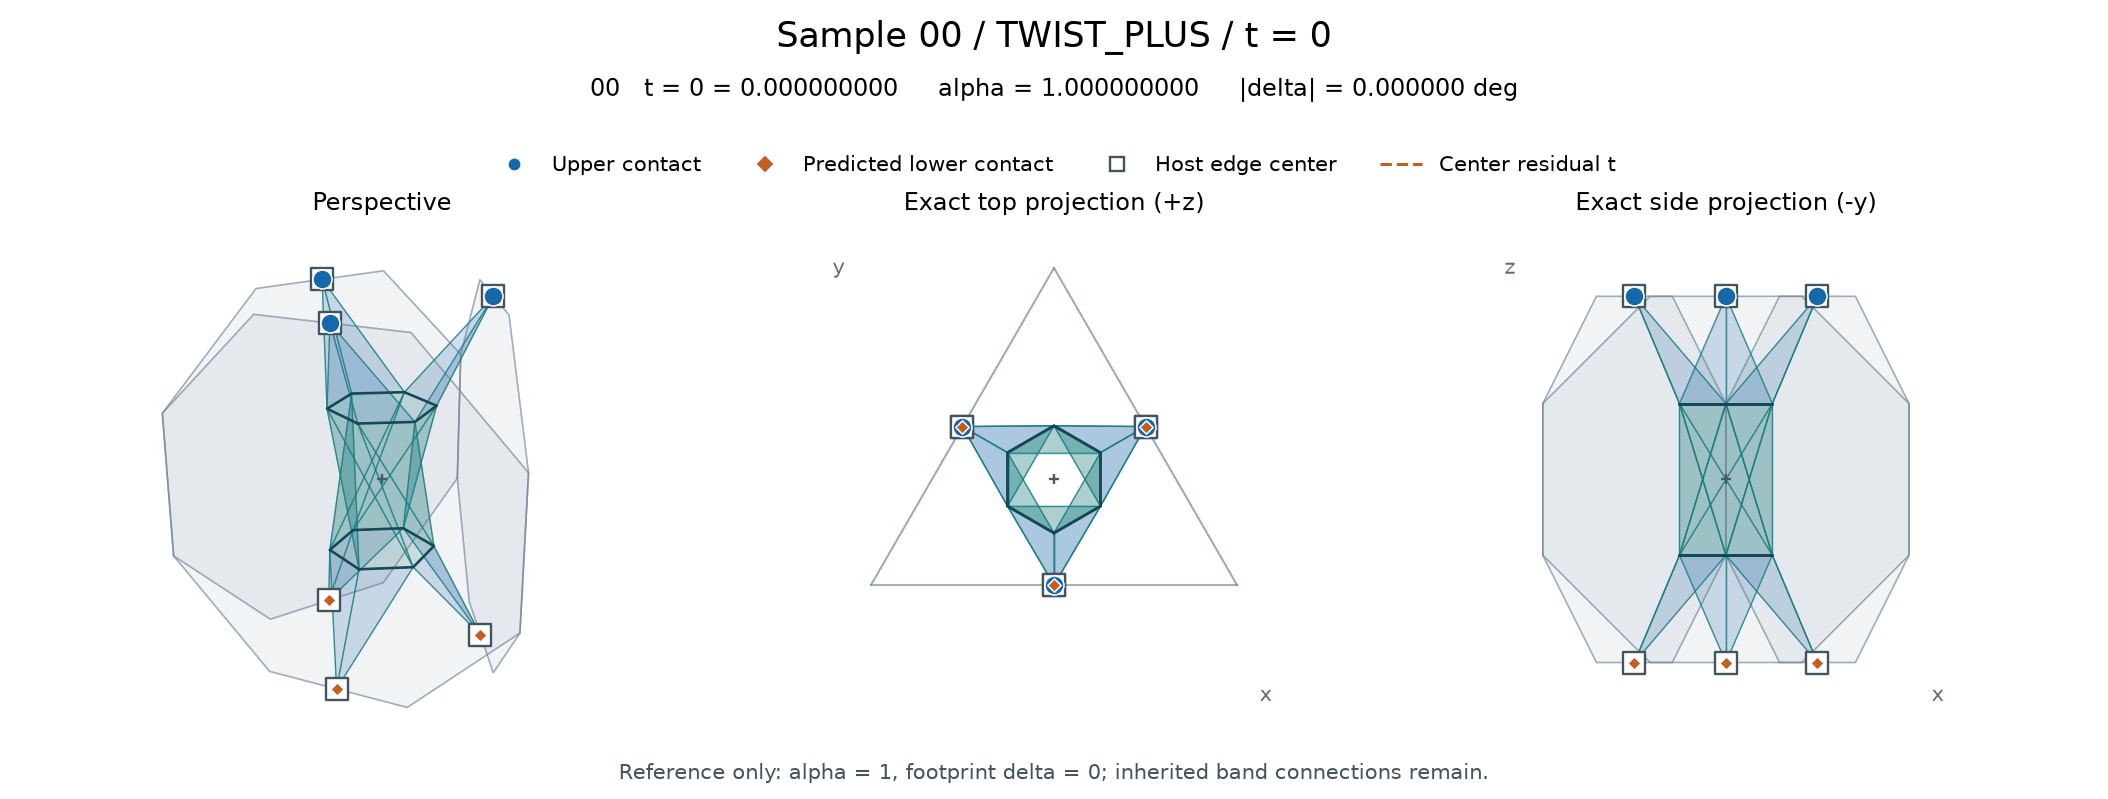
\includegraphics[width=\textwidth]{figures/zero_plus_retained.png}
\caption{Retained static atlas image of the PLUS zero member, at the accepted
width-one registration \cite{VisualAtlas}. The atlas's $t,\alpha,\delta$
mean this paper's crystal magnitude $\tau$, inverse planar scale, and footprint
angle. Thus $t=0$ here, not observer time. The cyan finite surface retains
the declared crossed band connections even though the ring footprints align.
The grey host and contact markers supply registration context. Projection
crossings are not a substitute for the face definitions in
\eqref{eq:faces}. No trajectory or mechanical turning path is depicted.}
\label{fig:zero}
\end{figure}

\begin{proposition}[Axial clearance]\label{prop:clearance}
Every point of either refined mesh has cylindrical radius at least $a/2>0$.
Every fan point satisfies $R_{\rm cyl}<|w|$.
\end{proposition}
\begin{proof}
The planar vertices of each face lie in an angular wedge of width at most
$2\pi/3$ and have radius at least $a$. Dotting with the wedge bisector gives
at least $a\cos(\pi/3)=a/2$ for every convex combination. For the upper fans,
the endpoint ratios are $a/h=1/\sqrt2$ and $r/H_0=1/\sqrt3$. Convexity of
the planar norm preserves the strict inequality relative to the linearly
interpolated positive height. On lower fans the ratios are multiplied by
$\sqrt{1+\xi^2}$. Their squared maxima satisfy
\[
\frac{a^2(1+\xi^2)}{h^2}\leq5-3\sqrt2<1,\qquad
\frac{r^2(1+\xi^2)}{H_0^2}\leq\frac13+s^2<1.
\]
Reflection does not change either radius or absolute height.
\end{proof}

\section{Actual sections and the finite constriction}\label{sec:sections}
Put $\eta=(1-w/h)/2$. Intersecting the actual faces, rather than interpolating
equal ring indices, gives
\begin{equation}\label{eq:sectionvertices}
S_i(\eta)=(1-\eta)ae_i+\eta aA_\tau e_{i+1},\qquad
D_i(\eta)=(1-\eta)ae_i+\eta aA_\tau e_{i+2}.
\end{equation}
At $0<\eta<1$, the twelve section edges are $S_iD_i$ and $D_iS_{i+1}$.
The section has $C_6$ symmetry although the complete surface has only $C_3$
in general. At the end levels these edges collapse in pairs to ring edges.
The points $(1-\eta)ae_i+\eta aA_\tau e_i$ are not this section.

\begin{theorem}[Section area and throat]\label{thm:area}
Every interior section is a simple star-shaped polygon about the axis. With
$\mathscr A_0=3\sqrt3a^2/2$, its area is
\begin{equation}\label{eq:area}
\mathscr A(\eta)=\mathscr A_0\left[
(1-\eta)^2+(1+\xi^2)\eta^2+
\frac{4\xi}{\sqrt3}\eta(1-\eta)\right].
\end{equation}
Let $p=1-2\xi/\sqrt3$ and $D=2+\xi^2-4\xi/\sqrt3=2p+\xi^2$.
Throughout $0\leq\tau\leq h$, $p,D>0$, and the unique minimum is
\begin{equation}\label{eq:throat}
\eta_*=\frac pD,\qquad
w_*=\frac{h\xi^2}{D},\qquad
\mathscr A_{\min}=\mathscr A_0\left(1-\frac{p^2}{D}\right)
\geq\frac{\mathscr A_0}{2}>0.
\end{equation}
The formula and throat height are the same for both hands.
\end{theorem}
\begin{proof}
Write $b=a\sqrt{1+\xi^2}$. Consecutive determinants are
\[
\det(S_i,D_i)=\frac{\sqrt3}{2}(\eta b)^2+
\eta(1-\eta)ab\sin\delta,
\]
\[
\det(D_i,S_{i+1})=\frac{\sqrt3}{2}((1-\eta)a)^2+
\eta(1-\eta)ab\sin\delta.
\]
They are positive for $0<\eta<1$, including $\xi=0$. Their angular sectors
assemble in the stated cyclic order with one winding, so the polygon is
simple and each ray meets its boundary once. The shoelace formula is three
times their sum; $b\sin\delta=a\xi$ gives \eqref{eq:area}.
The bracket is $1-2p\eta+D\eta^2$.
Since $\xi\leq\sqrt3s$, $p\geq1-2s>0$; also $D=2p+\xi^2>p$.
Completing the square proves the unique interior minimum. Finally,
$D-2p^2=2p(1-p)+\xi^2\geq0$ because $0<p\leq1$.
\end{proof}

At zero, $\eta_*=1/2$ and $w_*=0$. At $\tau=h$,
$\eta_*=1/5$, $w_*=3h/5$, and
$\mathscr A_{\min}=\mathscr A_0(1-s^2/5)$.
Thus a universal throat at the central plane would be incorrect.

\subsection{Inner and surrounding spaces}
In the slab $|w|<h$ the host cross-section is an equilateral support triangle
with inradius $r$ and area $\sqrt3/4$. The band section lies strictly inside
its incircle because $a\sqrt{1+\xi^2}<h<r$. Consequently
\begin{equation}\label{eq:complement}
\mathscr A_{\rm ext}(w)=\frac{\sqrt3}{4}-\mathscr A(w)
\end{equation}
has a maximum at the inner throat. This surrounding cross-section is a
connected annular region, not three disconnected channels.

An area constriction is therefore established for the inner finite slab.
A Venturi or Bernoulli conclusion is not: there is no specified fluid,
pressure, conserved flux, impermeable wall model, or inlet/outlet problem.
The surface is open, and its fan openings are additional geometry outside
the central slab. Area alone determines neither velocity nor transport
direction. This is the precise geometric content of the passage analogy.

\section{Fans, openings, and finite shell notches}\label{sec:openings}
Fan material, an opening between neighboring fans, a shell notch measurement
patch, and a material shell panel are four different sets. Put
$g_k=e_{2k+1}=n_k+n_{k+1}$ and $j_k=Jg_k$. The finite shell notch patch is
\begin{equation}\label{eq:notch}
\begin{aligned}
N_{k,\sigma}(\lambda_N,\zeta_N)
={}&\left(2r-\frac{\sqrt3d}{2}\lambda_N\right)g_k
+\zeta_Nj_k+\sigma(h+d\lambda_N)e_z,\\
&0\leq\lambda_N\leq1,\qquad
|\zeta_N|\leq d\lambda_N/2,\qquad \sigma=\pm1.
\end{aligned}
\end{equation}
Its plane is
\begin{equation}\label{eq:notchplane}
g_k\cdot(X,Y)+\sigma\frac{\sqrt3}{2}w
=2r+\frac{\sqrt3}{2}h.
\end{equation}
The displayed plus sign before $\zeta_Nj_k$ is essential. A point on this
infinite plane is not necessarily on the finite notch.

The upper opening boundary is the broken arc
$U_k-T_{2k+1}-U_{k+1}$. Its two side points at height $h+d\lambda_N$ are
\[
\left[(1-\lambda_N)a+\lambda_Nr/2\right]g_k
\ \pm\lambda_N\sqrt3r\,j_k/2.
\]
Its azimuthal bisector is $g_k$, the same as the upper notch, whereas the fan
tip is on $n_k$. These are alternating sets of three directions. The lower
opening is rotated by $-\delta$ and dilated by $\sqrt{1+\xi^2}$ in PLUS;
the host notch is fixed. Alignment of upper azimuths therefore does not imply
coincidence of the finite regions, and lower alignment varies with $\tau$.

For incidence, substitute vertices into the linear left side of
\eqref{eq:notchplane}. Upper fans are strictly on the inner side of every
upper notch plane. The maximum lower-tip value leaves the nonnegative
gap $\sqrt3(h-\tau)/2$; all lower-ring vertices are strictly inside.
Thus lower fans do not meet lower notch patches for $\tau<h$.
At $\tau=h$ the relevant lower tips meet notch vertices; there is no
positive-area fan/notch coincidence. Opposite-level patches are excluded by
height. This vertex-and-convexity argument concerns finite patches as defined
in \eqref{eq:notch}; it does not turn a measurement triangle into material
\cite[R2, Sections 3--4]{R2}.

\section{Traversal reversal and actual geometric operations}\label{sec:geomreverse}
\subsection{Reversing a line does not change its hand}
Each band cross-edge is
\[
\Gamma_{i,m}(\eta)=
\bigl((1-\eta)ae_i+\eta aA_\tau e_{i+m},\ h(1-2\eta)\bigr),
\qquad m=1,2.
\]
Its planar component never vanishes. On a continuous azimuth lift,
\begin{equation}\label{eq:edgeturn}
\frac{d\phi}{d\eta}
=\frac{a^2\sqrt{1+\xi^2}\sin(m\pi/3-\delta)}
{\abs{(1-\eta)ae_i+\eta aA_\tau e_{i+m}}^2}>0,\qquad
\frac{dw}{d\eta}=-2h.
\end{equation}
Here $0\leq\delta<\pi/3$. Traversing the same edge with decreasing $\eta$
reverses both derivatives and preserves their ratio. No reflection or
change of $\tau$ is needed. The same distinction applies to reversing a
piecewise fan-boundary arc.

\subsection{Face-level actions at zero and their obstruction away from zero}
Use the centered matrices
$H=\diag(1,1,-1)$, $S=\diag(-1,1,1)$,
$Q=SH=\diag(-1,1,-1)$, and $R=R_{2\pi/3}$ about the axis.
At $\tau=0$, $Q$ is a proper half-turn preserving each hand, while $H$ and
$S$ exchange hands. Actual face correspondences, with a superscript minus
denoting the reflected mesh, are
\begin{equation}\label{eq:faceactions}
\begin{array}{c|cc}
&F_i&D_i\\ \hline
H&D^-_{i+2}&F^-_{i+2}\\
S&F^-_{-i}&D^-_{-i}\\
Q&D_{-i-2}&F_{-i-2}.
\end{array}
\end{equation}
These follow by applying each matrix to the three vertices in
\eqref{eq:faces}, using $Se_i=e_{-i}$, and comparing the unordered triples.
For example $Q\Gamma_{i,m}(\eta)=\Gamma_{-i-m,m}(1-\eta)$.
$Q$ sends upper fan $k$ to lower fan $-k$ and upper opening arc $k$
to the reversed lower arc $-k-1$. On finite notches,
\[
H:(k,\sigma)\mapsto(k,-\sigma),\quad
S:(k,\sigma)\mapsto(-k-1,\sigma),\quad
Q:(k,\sigma)\mapsto(-k-1,-\sigma),\quad R:k\mapsto k+1.
\]
Substitution into \eqref{eq:notch} preserves both parameter inequalities.

For $\tau>0$, either $H$ or $Q$ would put the lower ring of radius
$a\sqrt{1+\xi^2}>a$ at the upper height. Every member in the registered
family has upper radius $a$. Hence that image is not another registered
member. The mirror $S$ still exchanges hands at the same $\tau$.

Finally, an axial rotation and translation preserving the exact upper three
contacts must have translation zero and rotation angle in $2\pi\mathbb Z/3$.
Continuity leaves only a constant such registered motion. This is a constraint
on a proposed motion with all contacts retained, not a statement that the
contacts are welded or a dynamical law. The zero half-turn is an endpoint
symmetry; it does not supply a feasible continuously registered turning path
\cite[R9, Sections 2--3]{R9}.

\clearpage
\part{How Z observations compare with the geometry}

\section{One native state, the staged observer, and placement}\label{sec:observer}
\subsection{Native update and readout definitions}
Let $\Omega=(\Omega_1,\Omega_2,\Omega_3)=x+\ii y\in\C^3$ and
$\Params=(\epsilon,g,\lambda,k_1,k_2,k_3)$. With $\Lmat$ having diagonal
$-2$ and off-diagonal $1$, the complete update is
\begin{equation}\label{eq:native}
\begin{aligned}
V=\Gmap_{\Params}(\Omega)
&=\Omega+\epsilon\,\Omega\odot(k-|\Omega|^2)+g\Lmat\Omega,\\
\Delta_j&=\lambda\sum_{m\ne j}\sin\bigl(3(\phi_m-\phi_j)\bigr),
\qquad \phi_j=\Arg V_j,\\
\Omega_j^+=\Fmap_{\Params}(\Omega)_j
&=|V_j|\exp\bigl(\ii(\phi_j+\Delta_j)\bigr).
\end{aligned}
\end{equation}
All $\Delta_j$ use the same pre-synchronization phases. The source convention
is $\Arg0=0$, including that phase in neighboring sums. When $\lambda=0$
the source bypasses synchronization. The nonzero-component arguments later
in the paper explicitly state their domains. Observer time increments are
not factors in \eqref{eq:native} \cite{PaperA,Native}.

Define
\begin{equation}\label{eq:readouts}
\begin{gathered}
\kappa=\norm{\Omega},\qquad
\chiral=x\times y=
\bigl(\Im(\overline\Omega_2\Omega_3),
\Im(\overline\Omega_3\Omega_1),
\Im(\overline\Omega_1\Omega_2)\bigr),\\
K(\kappa)=0.618\,\frac{\kappa}{1+\kappa},\quad
A(\kappa,t_c)=K(\kappa)\e^{-0.577t_c},\quad
f(\theta)=\cos3(\theta-\ell),\quad \ell=0.244,\\
d_\theta=(\cos\theta,\sin\theta,1),\qquad
\macro=A f(\theta)d_\theta,\qquad
\zobs=\alpha\macro+\beta\chiral .
\end{gathered}
\end{equation}
The existing weights are $\alpha=1,\beta=1/2$.
The macro amplitude and the chiral vector depend on the \emph{same} state;
they are not freely adjustable inputs to a fit. The area identity
\[
\norm{\chiral}^2=\norm{x}^2\norm{y}^2-(x\cdot y)^2
\leq\kappa^4/4
\]
is the Gram determinant and the elementary arithmetic--geometric mean
inequality \cite{PaperB,Atlas4}. The dimensionless passive ratio
$\chi=2\norm{\chiral}/\kappa^2$ is defined for $\kappa>0$.

The staged schedule uses twelve sectors, $m_n=n\bmod12$,
$\theta_n=m_n\pi/6$, and $t_{c,n}=0.1n$. First observe the given state at
$n=0$; then update the state, advance the clock and time, and observe.
Thus the $n$th scheduled observation uses exactly $n$ native updates.
The committed historical EMA observer is a different law and is not used
here \cite{PaperE,Atlas6}.

\subsection{Spatial meaning is declared}
The comparisons in Sections~\ref{sec:macro}--\ref{sec:case} use
\begin{equation}\label{eq:placement}
\Phi(\zobs)=O+\mu R_\psi\zobs,\qquad \mu>0,
\end{equation}
with an axial rotation $R_\psi$. Centered height is the third component of
$\mu R_\psi\zobs$. The worked certificate fixes $\mu=1,\psi=0$ and PLUS
$\tau=0$. Channel indices in $\Omega$ are not automatically spatial axes
under every shell symmetry; Section~\ref{sec:zsymmetry} tests that issue.
Anisotropic fitting is not introduced.

\section{Cone contact, frozen curves, and discrete samples}\label{sec:macro}
\begin{theorem}[Cone--band crossing]\label{thm:cone}
For either hand and every $\tau\in[0,h]$, the double cone
$R_{\rm cyl}=|w|$ misses all fan triangles and meets the band once on
each half-ray $(t\cos\varphi,t\sin\varphi,\sigma t)$,
$t>0$, $\sigma=\pm1$. Write this unique radius as
$T_\sigma(\varphi)\in(0,h)$. It is continuous and $C_6$-periodic.
\end{theorem}
\begin{proof}
Fan exclusion is Proposition~\ref{prop:clearance}. Write
$\mathcal R(w,\varphi)>0$ for the radial boundary of the star-shaped section.
At $w=0$ it is positive; at $w=\sigma h$ it is less than $h$, since the
largest ring radius is less than $h$. Continuity therefore gives a crossing.
For uniqueness, a section edge lies in a band face plane
$n_{xy}\cdot(X,Y)+n_ww=c_F$. With $k_0=\sqrt3/2$, valid outward data for
PLUS face index $i$ are
\begin{equation}\label{eq:bandplanes}
\begin{array}{c|ccc}
&n_{xy}&n_w&c_F\\ \hline
F_i&R_{\alpha_i}(k_0,1/2)&a(\xi-k_0)/(2h)&a(k_0+\xi)/2\\
D_i&R_{\alpha_i}(\xi,1)&a[k_0(1+\xi^2)-\xi]/(2h)&
a[k_0(1+\xi^2)+\xi]/2 .
\end{array}
\end{equation}
The constants and the supporting radial denominators
$n_{xy}\cdot e_\varphi$ are positive on their section edges. On each such
piece,
\[
\frac{\mathcal R(\sigma t,\varphi)}t
=\frac{c_F}{(n_{xy}\cdot e_\varphi)t}
-\frac{\sigma n_w}{n_{xy}\cdot e_\varphi}
\]
is strictly decreasing in $t$. It is continuous across edge changes;
the finite pieces establish uniqueness. Compactness and this unique crossing
give continuity; the sixfold section symmetry gives periodicity.
Reflection proves the other hand.
\end{proof}

This also corrects any argument based on corresponding-index ring
interpolation: the existence conclusion survives, but its proof uses the
actual triangles. Contact is with a finite face. For a candidate cone point
in a particular face,
\[
t=\frac{c_F}{n_{xy}\cdot e_\varphi+\sigma n_w}>0
\]
must additionally satisfy that triangle's barycentric inequalities
(Appendix~\ref{app:finite}).

\begin{theorem}[Frozen and sampled contact are different]\label{thm:frozen}
Freeze the native state and observer time with nonzero macro amplitude, put
$b=\mu\alpha A>0$, and $\vartheta=\ell+\psi$. The placed signed macro curve
meets band half $\sigma$ exactly when
\begin{equation}\label{eq:threshold}
b\geq B_\sigma,\qquad
B_\sigma=\min_{\cos3(\varphi-\vartheta)>0}
\frac{T_\sigma(\varphi)}{\cos3(\varphi-\vartheta)} .
\end{equation}
The minimum is attained and $a/2<B_\sigma<h$.
On the twelve-sector schedule with the default lock, the set of amplitudes
giving at least one exact sampled contact is the finite set
\begin{equation}\label{eq:discretecontact}
\bigcup_{\sigma=\pm1}
\left\{\frac{T_\sigma(\psi)}{\cos(0.732)},
\frac{T_\sigma(\psi+\pi/6)}{\sin(0.732)}\right\}.
\end{equation}
These conditions do not assert that every mathematical amplitude is reachable
under the bounded source amplitude and a fixed placement scale.
\end{theorem}
\begin{proof}
For either cone half, use the actual spatial azimuth. When the signed scalar
is negative this is $\varphi=\theta+\psi+\pi$, not $\theta+\psi$.
In both halves $t=b\cos3(\varphi-\vartheta)>0$.
On each positive-harmonic interval the quotient in \eqref{eq:threshold}
is continuous, tends to infinity at both ends, and has image $[B_\sigma,\infty)$.
Threefold repetition gives the same minimum. Clearance gives the lower
bound; equality at $a/2$ would require a limiting wedge midpoint at $w=0$,
which is not a nonzero cone contact. At a harmonic maximum the quotient
is $T_\sigma<h$, proving the upper bound. Above the minimum there are
at least two roots per positive interval, and at the minimum at least one.
On the clock, $f$ repeats $(c,s_\ell,-c,-s_\ell)$, where
$c=\cos(0.732)>0$ and $s_\ell=\sin(0.732)>0$.
Sixfold periodicity of $T_\sigma$ reduces all twelve samples to
\eqref{eq:discretecontact}.
\end{proof}

For example, if $b>h/\min(c,s_\ell)$ every discrete sample is beyond the
band although the continuous frozen curve has contacts. At $\tau=0,\psi=0$ a
concrete finite-face contact is available. Put
$k_*= \sqrt6/8$, $c_*=a\sqrt3/4$ (only in this paragraph),
$t_*=c_*/(1-k_*)$, and $\eta_*=(1-t_*/h)/2<1/3$.
Then $(t_*,0,t_*)\in F_1$ with barycentrics
$((1+\eta_*)/2,(1-3\eta_*)/2,\eta_*)$; the negative-height point is in
$D_0$ with the cyclic weights stated in Appendix~\ref{app:finite}.
Taking $b=t_*/c$ gives sampled contact. It is not the continuous threshold:
the quotient derivative at azimuth zero is $-3t_*s_\ell/c^2<0$
\cite[R1, Sections 4--6]{R1}.

\section{Full Z and the exact same-state contact witness}\label{sec:full}
For a frozen state and time, full Z translates the macro curve by
$\Delta_C=\mu\beta R_\psi\chiral$; its tangent with respect to angle is
unchanged by this translation. Consequently it need not lie on the original
macro cone, and the fan exclusion does not apply to it. A face contact solves
\begin{equation}\label{eq:fullface}
\mu\alpha A f(\theta)\,n\cdot R_\psi d_\theta
=c_F-n\cdot\Delta_C
\end{equation}
together with finite-face barycentrics. The undivided equation includes
zero harmonics and zero denominators. All harmonic zeros map to
$\Delta_C$, not necessarily to the origin.

The following construction realizes a fan point with the actual coupled
state variables; it does not vary $A$ and $\chiral$ independently.
At PLUS zero with identity placement, let
\begin{equation}\label{eq:contactstate}
\begin{gathered}
P=\left(\frac{\sqrt3a}{6},-\frac a2-\frac r3,
\frac{2h+H_0}{3}\right),\qquad A_*=0.4635,\qquad c=\cos(0.732),\\
c^\star=2\{P-A_*c(1,0,1)\},\qquad L=\norm{c^\star},\qquad
b_\perp=\sqrt{(c^\star_1)^2+(c^\star_2)^2},\\
p_0=(-c^\star_2,c^\star_1,0)/b_\perp,\qquad
q_0=(c^\star/L)\times p_0,\\
X=\sqrt{\frac{9+\sqrt{81-4L^2}}2},\qquad
Y=\sqrt{\frac{9-\sqrt{81-4L^2}}2},\qquad
\Omega_*=Xp_0+\ii Yq_0 .
\end{gathered}
\end{equation}
Here $0<L<4<9/2$ and $b_\perp>0$; the simple bounds in
Appendix~\ref{app:certificate} also certify them. The vectors $p_0,q_0$
are orthonormal, $X^2+Y^2=9$, and $XY=L$, so
\[
\norm{\Omega_*}=3,\qquad \chiral(\Omega_*)=c^\star,\qquad
\zobs(\Omega_*,0,0)=A_*c(1,0,1)+c^\star/2=P.
\]
$P$ is the centroid of $[U_0,T_0,T_1]$, with all three barycentric
weights $1/3$. This is an engineered exact witness, not a reconstructed
historical trajectory \cite[R2, Section 7]{R2}.

There is no universal extension of the macro amplitude threshold to full Z:
under scaling of a fixed state, the saturated macro factor stays bounded
while $\chiral$ scales quadratically. The same-state constraint remains
essential even when it permits a contact.

\section{The original input box through four updates}\label{sec:case}
\subsection{Hypotheses and the compact certificate}
Use the exact state \eqref{eq:contactstate}, not a decimal representative,
and reference tuple
\[
\Params_*=(0.1,0.2,0.17,2,3,4).
\]
Let $\boxinput$ be the closed Cartesian product in the six real state
coordinates $(x_1,x_2,x_3,y_1,y_2,y_3)$ and the six configuration coordinates:
every coordinate is within $10^{-8}$ of its reference value. Each chosen
$\Params$ is held identical across all updates. Geometry, placement, observer
weights, lock, and schedule are fixed. In particular $\tau=0$, so the
throat plane is $w=0$. Exact initial fan contact is required only of the
center, not of every perturbed input.

\begin{proposition}[Audited uniform four-update certificate]\label{prop:four}
For each input of $\boxinput$, apply exactly four complete native updates
\eqref{eq:native}. The resulting observations satisfy
Table~\ref{tab:observations}. Every observation after the initial one is inside
the host's central triangular prism; only observation one is inside the
band interior. Observations two, three, and four lie strictly outside its
finite boundary. In particular, the positive harmonic at observation four
does not restore band-interior membership.
\end{proposition}

\begin{table}[htbp]
\centering\small
\begin{tabular}{@{}clllll@{}}
\toprule
$n$ & $f(\theta_n)$ & Signed height $w_n$ & Axis distance & Center distance &
Band\\ \midrule
0 &$c$&$(.3046,.3049)$&$(.1693,.1760)$&$(.3484,.3530)$&above slab\\
1 &$s_\ell$&$(.16734,.16788)$&$(.10550,.1090)$&$(.1970,.2010)$&inside\\
2 &$-c$&$(-.1102,-.1075)$&$(.155,.160)$&$(.1886,.195)$&outside\\
3 &$-s_\ell$&$(-.0939,-.0926)$&$(.1387,.1401)$&$(.1667,.1687)$&outside\\
4 &$c$&$(.1333,.1370)$&$(.1247,.1301)$&$(.1825,.189)$&outside\\
\bottomrule
\end{tabular}
\caption{Uniform strict rational enclosures for the unchanged closed input
box. Throat-plane distance is $|w_n|$, not signed height. The first row
permits nearby points off the fan; its central input is the exact contact
witness. The first three rows inherit R4--R5, the last two R6; their scoped numerical checks are complete \cite{Audit,GPTAudit}.}
\label{tab:observations}
\end{table}

\begin{proof}[Proof and completed numerical check]
Appendix~\ref{app:certificate} gives the rational comparison states, residual
allowances, Lipschitz domains, and recurrences from R3--R6. The standalone
audit independently checked these inherited enclosures and their coverage
on the original closed box \cite{Audit}. The recurrences bound every input,
with its configuration fixed through all four updates.
Appendix~\ref{app:finite} carries the resulting coordinates through finite
section tests, including the directional test needed at observation four.
Those strict inequalities prove the classifications, not the harmonic signs.
The unchanged-checker replay reproduced the scalar certificates exactly
\cite{GPTAudit}; the implementation qualifications in
Appendix~\ref{app:crosswalk} still apply.
\end{proof}

All distance comparisons are with each input's own preceding observations.
From two to three, distances to the throat, axis, and center all decrease.
From three to four, the axis distance decreases but the throat and center
distances increase. Relative to observation one, observation four is closer
to the throat and center but farther from the axis. All four scheduled
endpoints are closer to the throat than their own initial observations.
These claims follow from disjoint intervals, without comparing different
inputs at selected midpoint values.

The first update also separates a native-only endpoint from a scheduled
endpoint. Let
$\zobs_N=\zobs(\Omega^+,t_c=0,\theta=0)$.
Uniformly it has $w_N\in(.19192,.19245)$ and radius greater than
$a+.00197$, while the scheduled endpoint has radius less than $.109$ and
lies inside a section of inradius greater than $.1144$.
Both remain above and closer to $w=0$ than their own initial observation:
$w_0>w_N>w_1>0$. This is the local robustness result of R4, with no exact
initial contact imposed on perturbations.

The table is a local finite certificate. It is not a basin, a general
stability result, or a continuous curve passing through successive openings.
No interpolation between observations is a native trajectory in the source.

\subsection{Native, envelope, and clock contributions}\label{sec:attribution}
Let $E=\e^{-.0577}$, $K_n=K(\kappa_n)$, $f_n=f(\theta_n)$, and
$d_n=d_{\theta_n}$. The exact telescoping split is
\begin{equation}\label{eq:attribution}
\begin{aligned}
\zobs_{n+1}-\zobs_n
={}&E^nf_n(K_{n+1}-K_n)d_n
+\frac{\chiral_{n+1}-\chiral_n}{2}\\
&+K_{n+1}E^n(E-1)f_nd_n\\
&+K_{n+1}E^{n+1}(f_{n+1}d_{n+1}-f_nd_n).
\end{aligned}
\end{equation}
These terms change the norm-derived amplitude, then chirality, then the
envelope, then the clock. The first two together are the native-only change.
Using the inherited bounds, their vertical sum is
$(-.00549,-.00395)$ from two to three and $(-.03027,-.02646)$ from three
to four. The corresponding envelope changes are $(.00747,.00754)$ and
$(.00697,.00707)$; the clock changes are $(.01277,.01287)$ and
$(.2485,.2509)$. In both transitions the native-only vertical change is
negative. The scheduled increases in signed height are therefore not native
upward forcing. In the fourth observation the positive clock term is decisive
for the sign, while finite geometry still determines exterior status.

\section{Symmetry residuals and conditional correspondences}\label{sec:zsymmetry}
\subsection{Macro identities at equal state and time}
Freeze $\Omega,t_c$ and write $A=A(\kappa,t_c)$. Direct trigonometry gives
\begin{equation}\label{eq:macroactions}
\begin{aligned}
\macro(\theta+\pi)&=H\macro(\theta),&
\macro(\theta+2\pi/3)&=R\macro(\theta),\\
\macro(\pi-\theta)-S\macro(\theta)
&=-2Ac\cos3\theta\,d_{\pi-\theta},\\
\macro(-\theta)-Q\macro(\theta)
&=2Ac\cos3\theta\,d_{-\theta}.
\end{aligned}
\end{equation}
On the twelve-sector grid these relabel $m$ as $m+6,m+4,6-m,-m$.
The latter two residuals vanish at odd sectors and generally not at even
ones. Reflection through the lock-dependent angle $\ell$ instead gives an
exact continuous macro identity, but its clock index is
$12\ell/\pi-m$, not an integer with the default lock. Its axes also fail to
be the shell reflection axes. Reversing the parameter of any frozen curve
always reverses its traversal; it does not require a spatial symmetry.

\subsection{Native channel actions are separate objects}
Let $\mathcal K\Omega=\overline\Omega$, let $P$ swap channel slots one and
three, and let $P_c(\Omega_1,\Omega_2,\Omega_3)=(\Omega_3,\Omega_1,\Omega_2)$.
The shell-induced actions from the controlling channel convention are
\[
T_H=\mathcal K,\qquad T_S=-P\mathcal K,\qquad
T_Q=-P,\qquad T_R=P_c.
\]
Their chiral vectors are respectively
$-\chiral$, $P\chiral$, $-P\chiral$, and $P_c\chiral$, whereas the geometric
actions are $H\chiral,S\chiral,Q\chiral,R\chiral$. The distinction is an
ordinary proper/improper transformation issue: for a real matrix $B$,
$(Bx)\times(By)=\cof(B)(x\times y)$.

Conjugation commutes with the complete forward map at the same real
configuration, including the zero convention. Simultaneously permuting the
channels and their $k$ labels is a covariance. At a fixed configuration,
the mismatch below vanishes in particular when $Pk=k$ or $\epsilon=0$;
a general fixed-configuration permutation symmetry is not supplied by
the worked unequal-$k$ tuple:
\[
\Gmap_{\Params}(P\Omega)-P\Gmap_{\Params}(\Omega)
=\epsilon\,P\Omega\odot(k-Pk).
\]
Vanishing on a particular state does not establish a general covariance.
Multiplication by a common phase, in particular a minus sign, commutes with
synchronization on nonzero pre-sync components (or with the bypass
$\lambda=0$); it is not a blanket zero-component statement with
$\Arg0=0$. Cross-product transformation identities themselves do include
zeros. Finally, $\mathcal K\Fmap\mathcal K=\Fmap$, not $\Fmap^{-1}$:
forward-map commutation is not inverse-time evolution.

\begin{proposition}[Exact full-Z residuals]\label{prop:residual}
At equal observer time, with the angle relabels of
\eqref{eq:macroactions}, define
$\mathcal E_G=\zobs(T_G\Omega,\widehat\theta)-G\zobs(\Omega,\theta)$.
Then
\begin{equation}\label{eq:residuals}
\begin{aligned}
\mathcal E_H&=(-2\beta C_1,-2\beta C_2,0),\\
\mathcal E_Q&=2\alpha Ac\cos3\theta\,d_{-\theta}
+\beta(C_1-C_3,-2C_2,C_3-C_1),\\
\mathcal E_S&=-2\alpha Ac\cos3\theta\,d_{\pi-\theta}
+\beta(C_1+C_3,0,C_1-C_3),\\
\mathcal E_R&=\beta(P_c\chiral-R\chiral).
\end{aligned}
\end{equation}
Here $(C_1,C_2,C_3)$ are components of the single original state.
\end{proposition}
\begin{proof}
All listed state actions preserve $\kappa$, so they preserve $A$.
Subtract the geometric action from the new full observation, use
\eqref{eq:macroactions}, and insert the four chiral transformations above.
This proves the residuals without assuming a new native orbit.
\end{proof}

For $H$ with conjugation, an equal-time match holds exactly when
$C_1=C_2=0$; using the \emph{same} state instead requires $C_3=0$.
For $Q$ with its shell action $-P$, odd grid sectors match exactly when
$C_1=C_3$ and $C_2=0$. For $S$, odd sectors require $C_1=C_3=0$.
For the rotational generator $R$, equality holds precisely on the line
$\chiral=t(-(2+\sqrt3),1,1)$; simultaneous matching of both $R$ and $R^2$
requires $\chiral=0$.

A different comparison, $Q$ with conjugation, is useful but is not the
shell-induced state action:
\begin{equation}\label{eq:qconj}
\zobs(\mathcal K\Omega,-\theta)-Q\zobs(\Omega,\theta)
=2\alpha Ac\cos3\theta\,d_{-\theta}-(0,2\beta C_2,0).
\end{equation}
For a nonzero state with the present positive weights, it vanishes on the
grid exactly at odd sectors with $C_2=0$. This provides a conditional
same-hand zero-mesh bridge. It does not supply a later observation: the
clock relabel $m\mapsto-m$ reverses order and does not commute with the
unchanged increment $+1$.

Appendix~\ref{app:residualcases} records the exceptional even-sector
cancellations. They are pointwise conditions, not all-grid symmetries.
The original witness has
$C_2=-a-2r/3<0$ and $C_3<0$, and it occurs at sector zero. It therefore
does not satisfy the $H$ bridges or the $Q$ conjugation bridge; the
shell-action $Q$ match at sector zero is impossible for any nonzero state.
It is not legitimate to replace that witness by a different state satisfying
the desired match.

If a residual vanishes and an observation already lies on a specified finite
face or notch, applying the geometric map transports its barycentric or
notch parameters and proves membership in the mapped finite region. This
is a contact implication. It neither establishes the existence of such a
contact under the special chiral conditions nor selects an exit or a
physical direction of travel.

\clearpage
\part{Why the native contributions change}

\section{Norm and chiral-area mechanisms}\label{sec:mechanism}
\subsection{The complete finite norm budget}
Set $I_j=|\Omega_j|^2$, $H_\Omega=\Omega\odot(k-I)$,
$D_\Omega=\epsilon H_\Omega+g\Lmat\Omega$, and
$J_\Omega=\sum_{j<k}|\Omega_j-\Omega_k|^2$. Synchronization preserves each
pre-sync magnitude, so expansion of the squared norm gives the exact identity
\begin{equation}\label{eq:normbudget}
\kappa_+^2-\kappa^2
=\underbrace{2\epsilon\sum_j I_j(k_j-I_j)}_{\mathcal O}
\underbrace{-2gJ_\Omega}_{\mathcal G}
+\underbrace{\norm{D_\Omega}^2}_{\mathcal R}.
\end{equation}
Here $\Re\ip{\Omega}{\Lmat\Omega}=-J_\Omega$.
The nonnegative finite-increment term must be retained; this is a discrete
identity, not a first-order differential approximation. Further,
\begin{equation}\label{eq:remainder}
\mathcal R=\epsilon^2\norm{H_\Omega}^2+
2\epsilon g\Re\ip{H_\Omega}{\Lmat\Omega}
+g^2\norm{\Lmat\Omega}^2,\qquad
\norm{\Lmat\Omega}^2=3J_\Omega .
\end{equation}
The last identity follows from $\Lmat^2=-3\Lmat$.
These are standard norm expansions, already used for this model in
\cite[Section 17]{PaperE} and implemented as diagnostics in \cite{Native}.

\begin{table}[htbp]
\centering\small
\begin{tabular}{@{}cllll@{}}
\toprule
Transition&$\mathcal O$&$\mathcal G$&$\mathcal R$&
$\kappa_{n+1}^2-\kappa_n^2$\\ \midrule
$1\to2$&$(.16900,.16924)$&$(-.27310,-.27283)$&$(.03635,.03653)$&
$(-.06775,-.06706)$\\
$2\to3$&$(.14654,.14711)$&$(-.16500,-.16426)$&$(.02510,.02562)$&
$(.00664,.00847)$\\
$3\to4$&$(.15774,.16009)$&$(-.10210,-.09942)$&$(.02250,.02509)$&
$(.07814,.08576)$\\
\bottomrule
\end{tabular}
\caption{Uniform inherited R7 norm budgets on $\boxinput$, with the complete
fixed-per-input update. Allowances are given in Appendix~\ref{app:mechanism}.}
\label{tab:budget}
\end{table}

The first transition contracts because its pairwise penalty dominates.
From two to three, $\mathcal O+\mathcal G\in(-.01846,-.01715)$ is still
negative, and the squared finite increment is essential to growth.
From three to four, $\mathcal O+\mathcal G\in(.05564,.06067)$ is already
positive; the remainder increases it further. The dominant onsite
contribution is channel three, followed by two and one. The two large
pair differences involving channel one decrease strongly before the latter
transition; the small $23$ difference increases. The mixed term in
\eqref{eq:remainder} is negative in all three rows, so the remainder is not
interpreted as a sum of three positive mechanisms.

\subsection{Pre-sync transport and simultaneous phase change}
At a fixed state, the polynomial stage is $V=\Bmat\Omega$ with the real
matrix
\[
\Bmat=\diag(1+\epsilon(k-I))+g\Lmat .
\]
It follows exactly that
\begin{equation}\label{eq:cofactor}
\chiral(V)=\cof(\Bmat)\chiral(\Omega).
\end{equation}
The cofactor identity is valid even when $\Bmat$ is singular. $\Bmat$
depends on the state and is not the Jacobian of the nonlinear update.

For a cyclic pair $(j,k)$ write
$\overline V_jV_k=P_{jk}+\ii A_{jk}$ and
$d_{jk}=\Delta_k-\Delta_j$. Simultaneous synchronization gives
\begin{equation}\label{eq:pairchange}
C_i^+=A_{jk}\cos d_{jk}+P_{jk}\sin d_{jk},\qquad
C_i^+-C_i(V)=A_{jk}(\cos d_{jk}-1)+P_{jk}\sin d_{jk}.
\end{equation}
This separates polynomial changes from the rotation of all pair products
by the already computed phase increments.

\begin{table}[htbp]
\centering\small
\begin{tabular}{@{}cllll@{}}
\toprule
State&$C_3$&$\norm{\chiral}$&$\chi=2\norm{\chiral}/\kappa^2$
&$C_3/\norm{\chiral}$\\ \midrule
$\Omega_2$&$(.04689,.04712)$&$(.0745,.0749)$&$(.652,.659)$&$(.627,.632)$\\
$V_3$&$(.03798,.03827)$&$(.0622,.0627)$&$(.527,.534)$&$(.607,.614)$\\
$\Omega_3$&$(.04008,.04101)$&$(.0649,.0665)$&$(.550,.567)$&$(.608,.626)$\\
$V_4$&$(.03237,.03394)$&$(.0537,.0564)$&$(.335,.359)$&$(.584,.621)$\\
$\Omega_4$&$(.00515,.00924)$&$(.0086,.0150)$&$(.053,.096)$&$(.592,.620)$\\
\bottomrule
\end{tabular}
\caption{Inherited R7 stage separation. $C_3$ is a signed component;
$\norm{\chiral}$ is full magnitude. The last two columns describe scale-free
area and one directional projection, respectively.}
\label{tab:chiral}
\end{table}

In update three, the polynomial stage lowers $C_3$ by
$(-.00914,-.00862)$ and synchronization raises it by $(.00218,.00268)$;
the net change remains $(-.00696,-.00594)$. Full magnitude also decreases
before synchronization and increases during it, with a net decrease.
In update four, both stages lower $C_3$, by $(-.00864,-.00614)$ and
$(-.02800,-.02400)$, giving $(-.03586,-.03084)$. Full magnitude decreases
in both stages. These conclusions survive division by the positive
stage norms as shown by the $\chi$ column.

Direction is a separate question. The separated ratios in
Appendix~\ref{app:mechanism} establish changes of direction at each of the
two stages. The complete transition from two to three decreases the
vertical fraction and therefore changes direction. The sign of the
vertical-fraction change during the third synchronization, during either
stage of the fourth update, and over the complete fourth update remains
unresolved by the inherited bounds. The net direction change from three
to four is also unresolved: two stage changes could partly undo each other.
Overlapping intervals do not show mixed behavior. In particular, a falling
$C_3$ cannot by itself be described as either a pure rotation or a pure
loss of area. Equations~\eqref{eq:attribution} and \eqref{eq:pairchange}
keep these native effects separate from the observer clock.

\section{Finite phase domains for synchronization gain and loss}\label{sec:phase}
\subsection{Exact two-phase reduction}
Assume $V_j=r_j\e^{\ii\phi_j}$ with every $r_j>0$, and choose continuous
local phase lifts. Define $u=\phi_2-\phi_1$, $v=\phi_3-\phi_2$, and
$\zeta=u+v/2$. Subtracting the simultaneous increments in
\eqref{eq:native} gives
\begin{equation}\label{eq:relative}
\begin{aligned}
u'&=u+\lambda[-2\sin3u+\sin3v-\sin3(u+v)],\\
v'&=v+\lambda[\sin3u-\sin3(u+v)-2\sin3v].
\end{aligned}
\end{equation}
Sum-to-product identities then give
\begin{equation}\label{eq:meanphase}
\boxed{\ \zeta'=\zeta-3\lambda\sin3\zeta\cos(3v/2)\ },\qquad
\boxed{\ v'=v-2\lambda\sin(3v/2)
[\cos3\zeta+2\cos(3v/2)]\ }.
\end{equation}
The sum $\sum_j\Delta_j=0$ is automatic from pair antisymmetry.
Changing lifts by $u\mapsto u+2\pi a$, $v\mapsto v+2\pi b$ changes
$\zeta$ by $2\pi a+\pi b$; the displayed phase rectangles use fixed local
lifts, not globally identified real angles.

Where $\lambda>0$ and $\cos(3v/2)>0$, the mean moves downward below
$\zeta=\pi/3$ and upward above it in the neighboring intervals.
The line itself is invariant under synchronization. This statement is about
the mean increment; it is neither invariance under $\Gmap$ nor a chiral-area
criterion.

\begin{theorem}[Exact weighted finite-step criterion]\label{thm:weighted}
For any positive magnitudes and any real lifted phases, set
$w_{jk}=r_j^2r_k^2$. Then synchronization increases, preserves, or decreases
full chiral magnitude according as
\begin{equation}\label{eq:weighted}
\begin{aligned}
\mathcal D={}&w_{12}\{\sin^2u'-\sin^2u\}
+w_{23}\{\sin^2v'-\sin^2v\}\\
&+w_{13}\{\sin^2(u'+v')-\sin^2(u+v)\}
\end{aligned}
\end{equation}
is positive, zero, or negative.
\end{theorem}
\begin{proof}
In cyclic component order,
\[
\chiral=(r_2r_3\sin v,\,-r_1r_3\sin(u+v),\,r_1r_2\sin u).
\]
Squaring and subtracting gives exactly
$\mathcal D=\norm{\chiral^+}^2-\norm{\chiral}^2$.
For bounding any summand use
$\sin^2b-\sin^2a=\sin(b+a)\sin(b-a)$.
Taking square roots preserves the sign of the squared-norm comparison.
\end{proof}

\subsection{Explicit closed domains}\label{sec:domaintheorems}
Write
\begin{equation}\label{eq:domains}
\begin{array}{c|cc|ccc}
&u&v&r_1&r_2&r_3\\ \hline
\mathcal S_3\times\mathcal A_3&
[1.214,1.223]&[.0404,.0447]&[.140,.144]&[.284,.289]&[.362,.369]\\
\mathcal S_4\times\mathcal A_4&
[.587,.614]&[.020,.038]&[.174,.181]&[.328,.335]&[.415,.424]
\end{array}
\end{equation}
and $\Lambda=[.16999999,.17000001]$.
These are Cartesian product hypotheses, including their endpoints, not
correlated samples of a trajectory.

\begin{theorem}[Uniform gain on the third domain]\label{thm:gain}
For all $(u,v,r,\lambda)\in\mathcal S_3\times\mathcal A_3\times\Lambda$,
\begin{equation}\label{eq:gainmargin}
\mathcal D>.00034.
\end{equation}
On $\mathcal S_3\times\Lambda$ without the magnitude box, a sufficient
gain condition is
$ .1(r_1/r_3)^2+.08(r_1/r_2)^2>.002$.
\end{theorem}
\begin{proof}
Here $\zeta\in[1.2342,1.24535]$ and $3v/2\in[.0606,.06705]$.
Writing $3\zeta=\pi+\alpha_0$ gives $.561<\alpha_0<.595$.
The alternating polynomial bounds detailed below give
\[
\begin{gathered}
.531<-\sin3\zeta<.561,\qquad -.847<\cos3\zeta<-.828,\\
\cos(3v/2)>.9977,\qquad
1.4988<\frac{\sin(3v/2)}v<1.5.
\end{gathered}
\]
Substitution into \eqref{eq:meanphase} yields
\[
.27018<\zeta'-\zeta<.28612,\quad
1.5043<\zeta'<1.5315,\quad .402<v'/v<.415,
\]
\[
.0162<v'<.0186,\quad 1.495<u'<1.524,\quad
1.512<u'+v'<1.541<\pi/2.
\]
Let $A_{12}=\sin^2u'-\sin^2u$, $A_{13}=\sin^2(u'+v')-\sin^2(u+v)$,
and $L_{23}=\sin^2v-\sin^2v'$. Bounding the cosine deficits from $\pi/2$
and the small-angle sines gives
\[
A_{12}>.3407^2-.0758^2=.11033085>.1,\quad
A_{13}>.2984^2-.0588^2=.08558512>.08,
\]
\[
.0012<L_{23}<.002.
\]
For the last pair, retain $v'<.415v$ and $\sin v>.99966v$:
$L_{23}>(.99966^2-.415^2)(.0404)^2>.0012$, while
$L_{23}<(.0447)^2<.002$.
Thus $\mathcal D>.1w_{12}+.08w_{13}-.002w_{23}$, proving the ratio
condition. On the full magnitude box the latter expression exceeds
\[
.1(.140\cdot.284)^2+.08(.140\cdot.362)^2
-.002(.289\cdot.369)^2
=.000340818146238>.00034 .
\]
All inequalities have strict slack on the closed product.
\end{proof}

\begin{theorem}[Uniform loss on the fourth domain]\label{thm:loss}
For all $(u,v,r,\lambda)\in\mathcal S_4\times\mathcal A_4\times\Lambda$,
\begin{equation}\label{eq:lossmargin}
\mathcal D<-.00248.
\end{equation}
For every $(u,v,\lambda)\in\mathcal S_4\times\Lambda$ and \emph{arbitrary}
strictly positive magnitudes, the sign remains negative. The fixed absolute
margin in \eqref{eq:lossmargin} requires the magnitude box.
\end{theorem}
\begin{proof}
Now $\zeta\in[.597,.633]$ and $3v/2\in[.030,.057]$. The same polynomial
bounds give
\[
\begin{gathered}
-.323<\cos3\zeta<-.218,\qquad .946<\sin3\zeta<.977,\\
\cos(3v/2)>.9983755,\qquad
\frac{\sin(3v/2)}v>1.49918775.
\end{gathered}
\]
Consequently
\[
.0987<\zeta'<.1514,\quad .091<v'/v<.147,\quad
.00182<v'<.005586,
\]
\[
.095<u'<.152,\qquad .099<u'+v'<.155.
\]
All three positive pair angles contract and remain below $\pi/2$.
Quantitatively,
\[
-A_{12}>.553^2-.152^2>.28,\quad
-A_{13}>.5697^2-.155^2>.30,\quad -A_{23}>.00039.
\]
The last bound uses the correlated inequality $v'<.147v$:
$-A_{23}>(.99975^2-.147^2)(.020)^2=.000391156425>.00039$,
since $\sin v>.99975v$ throughout this rectangle.
Thus $\mathcal D<-.28w_{12}-.00039w_{23}-.30w_{13}<0$ for all positive
magnitudes. On $\mathcal A_4$ the loss is greater than
\[
.28(.174\cdot.328)^2+.00039(.328\cdot.415)^2
+.30(.174\cdot.415)^2
=.002483531096736>.00248 .
\]
\end{proof}

\paragraph{Written bound method and review status.}
The theorem proofs use the finite rectangles, not the outcome table.
The rational trigonometric bounds are inherited from R8, Section 4, with
their sign and endpoint logic reviewed here. For $0\leq t\leq.61$,
the degree-seven alternating sine polynomial $S_7$ satisfies
$S_7(t)\leq\sin t\leq S_7(t)+t^9/9!$, with remainder below
$3.3\,10^{-8}$; the degree-eight cosine polynomial has error at most
$t^{10}/10!<2\,10^{-9}$. Reduce about $\pi$ or $\pi/2$ using
$3.1415926<\pi<3.1415927$ and parity, then apply these polynomials.
These estimates justify the outward strict bounds displayed above.
The final rational margin expansions are checked in writing in the review
notes. Their subsequent whole-domain interval checks are recorded in the completed audit \cite{Audit}; this document pass runs no evaluator.

\subsection{Why the mean line is not the response boundary}
Throughout this subsection take $\lambda\in\Lambda=[.16999999,.17000001]$.
The weights in \eqref{eq:weighted} and the finite phase step both matter.
On the invariant line $\zeta=\pi/3$, take $v\in[.02,.04]$ and
$r_2=r_3=\rho>0$. Then $.489<v'/v<.493$ and
\begin{equation}\label{eq:meanlineexample}
\mathcal D=\rho^2(\cos v'-\cos v)
\left[\frac{r_1^2}{2}-\rho^2(\cos v'+\cos v)\right],
\qquad 1.9984<\cos v'+\cos v<2.
\end{equation}
It is negative for $r_1=\rho$ and positive for $r_1=3\rho$ on the same
mean line. These are analytic comparisons of the existing map, not new
native trajectories. Likewise, on the slice $v=0$,
$\mathcal D=r_1^2(r_2^2+r_3^2)\sin(\zeta'+\zeta)\sin(\zeta'-\zeta)$.
At $\zeta=\pi/2$, the positive mean increment $3\lambda$ lowers $\sin^2\zeta$
by overshooting its maximum. A direction of mean movement alone cannot
replace the finite-step criterion.

\subsection{Separate inclusion of the actual certified inputs}\label{sec:inclusion}
The preceding domain theorems are independent of the four-update trajectory.
To apply them to that trajectory, R6--R8 supply additional information.
Their comparison pre-sync vectors and the propagated full-box radii imply
\begin{equation}\label{eq:actualphase}
\begin{array}{c|cc|c}
&u&v&\text{pre-sync complex-component radius}\\ \hline
V_3&(1.214487,1.221613)&(.040439,.044611)&<.00032\\
V_4&(.58711,.61399)&(.02075,.03755)&<.00151 .
\end{array}
\end{equation}
Their magnitudes lie in $\mathcal A_3,\mathcal A_4$ and each input's
coefficient lies in $\Lambda$. The intervals are strictly within
\eqref{eq:domains}. Appendix~\ref{app:inclusion} exhibits the argument-error
allowances. This inclusion inherits the nominal residual chain, separately
checked with its original-box application in the subsequent audit
\cite{Audit,GPTAudit}. Reuse of R6 in R7 and R8 alone was not that check.

After the third synchronization, $\zeta'>1.5043>\pi/3$. The next polynomial
stage supplies $V_4$ with $\zeta<.633<\pi/3$ before the same synchronizer is
applied again. The polynomial update, rather than a change in $\lambda$,
therefore supplies the different domains. In its first component, the
own-state and neighbor real contributions are respectively
$(.14999,.15038)+(-.10174,-.10154)$ for $V_3$, and
$(.05675,.05848)+(-.10890,-.10802)$ for $V_4$.
The imaginary components are positive. The first pre-sync phase changes
from quadrant I to quadrant II while the other two remain in quadrant II.
Arguments of sums are not sums of arguments; the displayed signed sums
explain the domain change without making that invalid replacement.

\section{Synthesis}\label{sec:synthesis}
The refined geometry provides an open finite surface, positive axial
clearance, a precisely located inner area minimum, and distinguishable
threefold fan openings and shell notches. At zero it admits a same-hand
upper/lower half-turn; away from zero the ring-size obstruction prevents
that correspondence within the registered family. Reversing a traversal
requires neither reflection nor shape change.

The existing Z readout has its own exact structure. Cone, frozen-curve,
and discrete contacts are different questions. A same-state chiral
translation permits the exact fan witness, but its four scheduled updates
do not describe a continuous passage, and the harmonic return does not
restore interior membership. Full-Z correspondence follows explicit
residual conditions rather than visual analogy.

The native mechanisms are equally specific: the finite-increment norm
remainder matters, polynomial and synchronization effects on chirality
can oppose or reinforce each other, and the weighted finite-step criterion
has explicit domains of strict gain and loss. The locally uniform example
illustrates those mechanisms with the inherited enclosure chain and its
completed scoped audit distinguished \cite{Audit,GPTAudit}.
No crystal motion law, geometry-to-native feedback, transport equation, SRG
premise, or memory premise has been supplied by these results. This manuscript
ends at the existing fourth update for review.

\appendix

\section{Finite-region tests and the classification margins}\label{app:finite}
\subsection{A reusable triangle test}
For a triangle $[A,B,C]$, put $b=B-A$, $c=C-A$, $p=P-A$ and
$G=(b\cdot b)(c\cdot c)-(b\cdot c)^2>0$. A coplanar point belongs to
the finite triangle exactly when
\[
\lambda_B=\frac{(p\cdot b)(c\cdot c)-(p\cdot c)(b\cdot c)}G\geq0,\quad
\lambda_C=\frac{(p\cdot c)(b\cdot b)-(p\cdot b)(b\cdot c)}G\geq0,\quad
1-\lambda_B-\lambda_C\geq0.
\]
Strict inequalities give its relative interior. This test accompanies
every infinite-plane equation used in the text. At the explicit zero
cone witness in Section~\ref{sec:macro}, the positive point's weights on
$[T_1,T_2,B_3]$ are
$((1+\eta_*)/2,(1-3\eta_*)/2,\eta_*)$; the negative point's weights on
$[T_0,B_2,B_1]$ are
$(\eta_*,(1+\eta_*)/2,(1-3\eta_*)/2)$.

\subsection{Section tests for the four-update box}
At zero, all section vertices have radius
$a\sqrt{1-\eta+\eta^2}$ or the corresponding radius from the other
cross-edge; the maximum is $a\sqrt{1-\eta+\eta^2}$.
For observation two, the inherited radial lower bound $.155$ already exceeds
$a$ by more than $.0085$, excluding the whole band.

At observation three, the inherited Cartesian box is
\[
X_3\in(.0005,.0014),\quad Y_3\in(-.1400,-.1387),\quad
w_3\in(-.0939,-.0926).
\]
It gives $\eta_3\in(.723,.727)$ and an outer section radius less than
$.1313$. The actual point radius exceeds $.1387$, leaving more than
$.0074$ of radial separation.

At observation four,
\[
X_4\in(-.0675,-.0636),\quad Y_4\in(.1073,.1111),\quad
w_4\in(.1333,.1370),\qquad \eta_4\in(.169,.179).
\]
A global outer-radius test alone is insufficient. Its ray meets the finite
section edge $D_3S_4$ of $[T_3,T_4,B_5]$, since
\[
D_3=a(-k_0\eta,1-1.5\eta),\qquad
S_4=a(-k_0,.5-\eta),\qquad k_0=\sqrt3/2,
\]
\[
\det(D_3,(X_4,Y_4))/a
>.7315(.0636)-.8661(.179)(.1111)>.029,
\]
\[
\det((X_4,Y_4),S_4)/a
>.8660(.1073)-.0675(.331)>.0705.
\]
These signs place the ray between the endpoints. The outward unit normal
$n=(-1/2,k_0)$ then gives
\[
n\cdot(X_4,Y_4)>.1247218,\qquad
n\cdot D_3=n\cdot S_4=ak_0(1-\eta)<.1055.
\]
The residual exceeds $.0192$. This proves exterior status in the correct
finite angular sector, with radial separation greater than $.0192$.
It is not a claimed minimum distance to the entire band.

For the first native-only endpoint R4 gives
\[
X_N\in(.14847,.14900),\quad Y_N\in(-.04516,-.04479),\quad
w_N\in(.19192,.19245),
\]
so $R_N>a+.00197$. The scheduled first endpoint satisfies
$X_1\in(.10550,.10603)$, $Y_1\in(.02344,.023895)$ and the height in
Table~\ref{tab:observations}; its radius is $R_1<.109$.
At each input's own perturbed height put $\eta_1=(1-w_1/h)/2$.
For the actual zero-member section, the two triangle types give
\begin{equation}\label{eq:firstinradius}
\mathcal R(w,\varphi)\geq L(\eta)
=\min\left\{\frac{a\sqrt3(1-\eta)}2,\ a\left(1-\frac32\eta\right)\right\}.
\end{equation}
On a top-two-vertex triangle the projection on its unit horizontal plane
normal is $a\sqrt3(1-\eta)/2$; on a bottom-two-vertex triangle the projection
on $e_i$ is at least $a(1-3\eta/2)$. These projections bound every section
segment, including the inward vertices. Since the established star-shaped
section contains the axis, its filled interior contains the open disk of
radius $L(\eta)$ whenever both bounds are positive.
The inherited height and radical bounds give $0<\eta_1<.097$ and
\[
\frac{a\sqrt3(1-\eta_1)}2>.1464(.8660)(.903)>.1144,\qquad
a(1-3\eta_1/2)>.1464(.8545)>.1144.
\]
Thus $L(\eta_1)>.1144>R_1$, with an interior clearance greater than $.0054$,
at every input-dependent height and azimuth. This restores R4
Section~5.4, equations~(32)--(34); its numerical substitutions remain
inherited from R4 and subsequently checked \cite{R4,Audit}.
The disk is a consequence of the actual triangles,
not a replacement geometry. Both endpoints are inside the host because their radii are
less than $r$, and both satisfy $0<w_1<w_N<w_0$.

For all scheduled $n=1,\ldots,4$, $R_n<r$ and $|w_n|<h$ prove host
central-prism membership. Fan and notch points have $|w|\geq h$, so these
observations cannot lie on those finite sets. Their axis and center
distances are bounded from the Cartesian boxes by
$\sqrt{X_n^2+Y_n^2}$ and $\sqrt{X_n^2+Y_n^2+w_n^2}$ using rational
squaring. The distance intervals in the main table are intentionally wider
than the tightest possible ones.

\section{The inherited four-update enclosure chain}\label{app:certificate}
\subsection{Status and exact starting point}
This appendix records the load-bearing numerical chain of R3--R6.
The subsequent standalone audit checked its initial inclusion, comparison
residuals, nonzero-domain coverage, sensitivity estimates, and propagation
recurrences; GPT's unchanged-checker replay matched the saved records
\cite{Audit,GPTAudit}. The original bounds and source attributions are
retained. No change has been made to the original input uncertainty.

The exact initial state is \eqref{eq:contactstate}. A cancellation-free form is
\begin{equation}\label{eq:initialxy}
x=\left(-\frac{Xc^\star_2}{b_\perp},
\frac{Xc^\star_1}{b_\perp},0\right),\quad
y=\left(-\frac{c^\star_3c^\star_1}{Xb_\perp},
-\frac{c^\star_3c^\star_2}{Xb_\perp},\frac{b_\perp}{X}\right).
\end{equation}
R3 bounds
\[
\begin{gathered}
1.4142135<\sqrt2<1.4142136,\quad
1.7320508<\sqrt3<1.7320509,\\
.7438391<c<.7438393,\quad .6683<s_\ell<.6684,\quad .9439<E<.9440,\\
c^\star_1\in(-.6049883,-.6049877),\
c^\star_2\in(-.3388968,-.3388966),\
c^\star_3\in(-.0800636,-.0800629),\\
b_\perp\in(.69344,.69345),\qquad X\in(2.99090,2.99092).
\end{gathered}
\]
Roots are bounded by squaring rational endpoints. Cosine at $.732$ uses
alternating terms through degrees ten and eight, sine through seven and
nine, and $\exp(-.0577)$ through five and four. These are exact rational
arguments. R6 refines \eqref{eq:initialxy} to
\[
\begin{array}{c|ccc}
&1&2&3\\ \hline
x&(1.461705,1.461710)&(-2.609399,-2.609390)&0\\
y&(-.0233545,-.0233541)&(-.0130826,-.0130822)&(.2318496,.2318503).
\end{array}
\]

\subsection{Comparison centers and pre-sync residuals}
The following terminating decimals are rational \emph{comparison vectors},
not replacement initial data. A pair $(a,b)$ in this table denotes
$a+\ii b$, not an interval.
\begin{table}[htbp]
\centering\small
\begin{tabular}{@{}clll@{}}
\toprule
$n$&$\widehat\Omega_{n,1}$&$\widehat\Omega_{n,2}$&$\widehat\Omega_{n,3}$\\ \midrule
0&$(1.461707,-.0233543)$&$(-2.609395,-.0130824)$&$(0,.2318499)$\\
1&$(.322706,.095167)$&$(-.259081,.111445)$&$(-.244759,.206520)$\\
2&$(.188739,.085078)$&$(-.223602,.148232)$&$(-.284600,.179065)$\\
3&$(.072196,.121963)$&$(-.237006,.161219)$&$(-.305291,.199972)$\\
4&$(-.102612,.144250)$&$(-.223813,.244521)$&$(-.284466,.308622)$\\
\bottomrule
\end{tabular}
\caption{R6 rational comparison centers, with the exact initial state
within $.000006$ in maximum complex-component norm.}
\label{tab:centers}
\end{table}
\begin{table}[htbp]
\centering\small
\begin{tabular}{@{}clll@{}}
\toprule
$n$&$\widehat V_{n,1}$&$\widehat V_{n,2}$&$\widehat V_{n,3}$\\ \midrule
1&$(.3351004,.0300612)$&$(-.2793475,.0388329)$&$(-.2295376,.2233163)$\\
2&$(.153744,.138649)$&$(-.215523,.159751)$&$(-.229524,.245724)$\\
3&$(.048542,.133157)$&$(-.218805,.185171)$&$(-.288355,.223702)$\\
4&$(-.050848,.169564)$&$(-.257977,.208159)$&$(-.334187,.253945)$\\
\bottomrule
\end{tabular}
\caption{R6 pre-sync comparison centers. Each real and imaginary difference
from $\Gmap_{\Params_*}(\widehat\Omega_{n-1})$ is less than $.000002$;
the complex-component difference is less than $.000003$. These are
inherited polynomial residual bounds.}
\label{tab:precenters}
\end{table}

For example, at the exact initial state the nominal real matrix is
\[
\Bmat_*=\begin{pmatrix}
.8-.1I_1&.2&.2\\ .2&.9-.1I_2&.2\\ .2&.2&1-.1I_3
\end{pmatrix}.
\]
R3's wider direct certificate gives
\[
\begin{aligned}
V_{1,1}&\in(.33497,.33523)+\ii(.03005,.03008),\\
V_{1,2}&\in(-.27953,-.27916)+\ii(.03882,.03885),\\
V_{1,3}&\in(-.22958,-.22950)+\ii(.22330,.22334).
\end{aligned}
\]
It can use $\sin3\varphi=3\sin\varphi-4\sin^3\varphi$ on normalized
pair products instead of phase inversion. The refined R6 route below
uses small arctangent arguments to sharpen subsequent stages.

\subsection{Argument and synchronization residual allowances}
At the exact polynomial image of each comparison center, R6 encloses the
three small arguments $t_j$ as follows:
\begin{table}[htbp]
\centering\small
\begin{tabular}{@{}clll@{}}
\toprule
$n$&$t_1$&$t_2$&$t_3$\\ \midrule
1&$(.089706,.089711)$&$(.139012,.139016)$&$(.013736,.013741)$\\
2&$(.051620,.051628)$&$(.148613,.148624)$&$(.034083,.034092)$\\
3&$(.36453,.36457)$&$(.08325,.08327)$&$(.12625,.12628)$\\
4&$(.29986,.29989)$&$(.10686,.10689)$&$(.13642,.13646)$\\
\bottomrule
\end{tabular}
\caption{Inherited argument quotients at the exact polynomial images, not
at the rounded $\widehat V_n$.}
\label{tab:atan}
\end{table}
The phase triples are respectively
\[
\begin{array}{c|lll}
1&\arctan t_1&\pi-\arctan t_2&3\pi/4+\arctan t_3\\
2&\pi/4-\arctan t_1&3\pi/4+\arctan t_2&3\pi/4-\arctan t_3\\
3&\pi/2-\arctan t_1&3\pi/4+\arctan t_2&3\pi/4+\arctan t_3\\
4&\pi/2+\arctan t_1&3\pi/4+\arctan t_2&3\pi/4+\arctan t_3.
\end{array}
\]
The alternating arctangent polynomial through degree thirteen has error
less than $t^{15}/15<2\,10^{-8}$ for $t\leq.365$.
Reduce the triple angles about multiples of $\pi/4$; residual arguments
are less than $1.5$. Sine through degree thirteen and cosine through
twelve have errors less than $4\,10^{-9}$ there. The same bound suffices
for the smaller final increments. The resulting allowances are
\begin{table}[htbp]
\centering\small
\begin{tabular}{@{}cllll@{}}
\toprule
$n$&$\Delta_1$&$\Delta_2$&$\Delta_3$&
$\rho_n>\norm{\Fmap_{\Params_*}(\widehat\Omega_{n-1})-\widehat\Omega_n}_\infty$\\
\midrule
1&$(.19729,.19733)$&$(-.26812,-.26808)$&$(.07077,.07082)$&$.00002$\\
2&$(-.31035,-.31030)$&$(.05243,.05248)$&$(.25784,.25791)$&$.00004$\\
3&$(-.18495,-.18485)$&$(.10496,.10504)$&$(.07987,.07995)$&$.00005$\\
4&$(.32690,.32703)$&$(-.15071,-.15060)$&$(-.17636,-.17625)$&$.00005$\\
\bottomrule
\end{tabular}
\caption{Inherited simultaneous-increment and full-update residual bounds.
The displayed norm is maximum complex-component norm.}
\label{tab:residualbounds}
\end{table}

\subsection{Domains and Lipschitz propagation}
For an own-channel polynomial component, the real two-dimensional radial
and tangential derivative eigenvalues are
$1-2g+\epsilon(k_j-3I_j)$ and $1-2g+\epsilon(k_j-I_j)$.
Together with the off-diagonal $g$ terms, these give a component maximum-norm
Lipschitz constant $1.6$ initially and $1.41$ in the later domains.

For synchronization, let $a_{jm}=\cos3(\phi_m-\phi_j)$. The row bound
used in R6 is
\begin{equation}\label{eq:synclip}
\max\left\{1,\left|1-3\lambda\sum_{m\ne j}a_{jm}\right|\right\}
+3|\lambda|\sum_{m\ne j}\frac{|V_j|}{|V_m|}|a_{jm}|.
\end{equation}
It follows by differentiating radial and angular coordinates on a convex
nonzero neighborhood, with $|d\phi_m|\leq |dV_m|/|V_m|$.
The relevant domains are
\begin{table}[htbp]
\centering\small
\begin{tabular}{@{}cllll@{}}
\toprule
$n$&$(r_1,r_2,r_3)$ intervals&$a_{12}$&$a_{13},a_{23}$&$L_n$\\ \midrule
1&all $(.28,.34)$&$[-1,1]$&$[-1,1],[-1,1]$&4\\
2&$(.206,.209),(.267,.270),(.334,.338)$&$(.45,.65)$&
$(-.10,.10),(.80,.90)$&2\\
3&$(.140,.144),(.284,.289),(.362,.369)$&$(-.91,-.82)$&
$(-.85,-.73),(.97,1]$&3.2\\
4&$(.174,.181),(.328,.335),(.415,.424)$&$(-.29,-.16)$&
$(-.39,-.23),(.98,1]$&2.6\\
\bottomrule
\end{tabular}
\caption{R6 nonzero domains and synchronizer constants. Their coverage must
be checked together with the recurrences, not assumed from later outcomes.}
\label{tab:lipdomains}
\end{table}

Let $e_n$ bound nominal distance from the comparison center.
The recurrence $e_n\leq L_nL_Ge_{n-1}+\rho_n$ admits
\[
(e_0,e_1,e_2,e_3,e_4)
=(.000006,.000060,.000220,.001050,.003900).
\]
The right sides before outward rounding are
$.0000584,.0002092,.00104264,.0038993$.

Now let $\delta_0=10^{-8}$ denote the \emph{original} input-coordinate
radius. The initial component perturbation is at most $\sqrt2\delta_0$.
R6's first-stage coefficient derivative sum is less than $21.27\delta_0$,
and the state term less than $2.4\delta_0$. It takes
$D_1=.00000025$ and $Q_1=.0000011$, including the
$.68\delta_0$ synchronizer-coefficient contribution.
At subsequent stages, the combined parameter derivative bound is
less than $1.9+1.8+.046<4$. Hence
\begin{equation}\label{eq:boxrecurrence}
D_n\leq1.41Q_{n-1}+4\delta_0,\qquad
Q_n\leq L_nD_n+2M_n\delta_0,
\end{equation}
where $M_n$ bounds pre-sync component magnitude. Valid outward choices are
\[
\begin{array}{c|cc}
n&D_n&Q_n\\ \hline
2&.0000016&.0000033\\
3&.0000047&.0000151\\
4&.0000214&.0000557 .
\end{array}
\]
The total radii about the rounded pre-sync centers, including the polynomial
residual $.000003$, are
\[
\begin{aligned}
1.41(.000060+.0000011)+.00000004+.000003
&=.000089191<.00009,\\
1.41(.000220+.0000033)+.00000004+.000003
&=.000317893<.00032,\\
1.41(.001050+.0000151)+.00000004+.000003
&=.001504831<.00151 .
\end{aligned}
\]
The last value corrects R6's printed $.001504871$, which was a slightly
larger conservative number; the domain containment is unchanged.

\subsection{Readout bounds and the earlier coarse proof route}
Norm preservation by synchronization makes the macro perturbation depend
on the smaller pre-sync radius. For the present weights,
each observation-component error is bounded by
$1.236D_n+M_nQ_n$; it is less than $.000012$ for $n=3$ and
$.000051$ for $n=4$. Representative nominal scalar bounds are
\[
\begin{array}{c|cc}
&n=3&n=4\\ \hline
\kappa_n&(.4845,.4860)&(.5603,.5664)\\
K_n\ \text{(uniform)}&(.20159,.20221)&(.22187,.22353)\\
\text{positive }K_nE^n|f_n|&(.1132,.1138)&(.1309,.1322).
\end{array}
\]
Uniform $\kappa_3\in(.48449,.48601)$ and
$\kappa_4\in(.56025,.56645)$ incorporate the box error.
Also $K_2\in(.19919,.20011)$,
$E^3\in(.8409,.8413)$, $E^4\in(.7937,.7942)$, and
$\sqrt3/2\in(.8660254,.86602545)$.
The comparison chiral vectors are
\[
\begin{aligned}
\widehat C_3&=(.001824145897,-.051671384745,.040545329702),\\
\widehat C_4&=(.000484295100,-.009365899836,.007194236398).
\end{aligned}
\]
Nominal enclosures are
$C_3\in(.0011,.0026)\times(-.0523,-.0511)\times(.0400,.0411)$ and
$C_4\in(-.0025,.0035)\times(-.0118,-.0070)\times(.0051,.0093)$.
Combining them with the amplitude and phase factors produces the Cartesian
boxes in Appendix~\ref{app:finite}.

R4 and R5 used broader bounds for the first two observations; the main table
retains those conservative early results rather than silently replacing
prior reports. In R4 the first pre-sync error is
$26\delta_0+52\delta_0=.00000078$; the post-sync error is
$21(.00000078)+\delta_0=.00001639$.
The observation error is at most
$1.236(.00000078)+.34(.00001639)=.00000653668<10^{-5}$;
the initial error is at most $9\delta_0$.
Adding this allowance to the nominal native-only and scheduled endpoints
gives the first-step intervals in Appendix~\ref{app:finite}.
R5 uses $D_2=.00004$, $Q_2=.00096001$, and
observation error $.0003758434<.0004$.
Its nominal second point lies in
$(-.0661,-.0641)\times(-.1446,-.1427)\times(-.1098,-.1079)$;
the larger uniform box is
$(-.0665,-.0637)\times(-.145,-.1423)\times(-.1102,-.1075)$.
These proof widths are not new perturbations of the original inputs.

\section{Mechanism bounds and unresolved direction projections}\label{app:mechanism}
R7 evaluates the exact budget \eqref{eq:normbudget} using the comparison
states and total radii
$t_n=e_n+Q_n=(.0000611,.0002233,.0010651)$ for $n=1,2,3$.
The rational comparison intensities are
\[
\begin{array}{c|ccc}
n&\widehat I_1&\widehat I_2&\widehat I_3\\ \hline
1&.113195920325&.079542952586&.102557478481\\
2&.042860676205&.071970580228&.113061434225\\
3&.020087235785&.082163409997&.133191395465 .
\end{array}
\]
The elementary bound $|I_j-\widehat I_j|\leq
2|\widehat\Omega_j|t_n+t_n^2$ (or $2M_jt_n$ with $M_j$ bounding the
whole segment) propagates into onsite channel errors
\[
(.000017,.000026,.000034),\quad
(.000038,.000073,.000122),\quad
(.000123,.000370,.000630),
\]
including parameter effects less than $2\,10^{-8}$. For a pair difference,
the square error is at most
$4|\widehat\Omega_j-\widehat\Omega_k|t_n+4t_n^2$.
The comparison pair sums are
$.682401478796,.411568322980,.251893385824$.
The two growth stages have individual pair-square enclosures
\[
\begin{array}{c|ccc}
&12&13&23\\ \hline
\Omega_2&(.17363,.17440)&(.23245,.23332)&(.00460,.00474)\\
\Omega_3&(.09581,.09849)&(.14693,.15024)&(.00582,.00651).
\end{array}
\]
Their onsite channel contributions are
$(.01673,.01683),(.04206,.04224),(.08775,.08804)$ and
$(.00782,.00809),(.04756,.04834),(.10236,.10366)$, respectively.

For the finite-increment remainder use
$\widehat D_n=\widehat V_{n+1}-\widehat\Omega_n$.
The component error is
$b_n\leq2.41t_n+4\delta_0+.000003$, with outward values
$.000150291,.000541193,.002569931$.
The comparison squared norms are
$.036438669609,.025360851774,.023796891123$ and the sums of component
moduli are less than $.284,.232,.246$.
Thus the squared-norm errors are at most
$2b_n\sum_j|\widehat D_{n,j}|+3b_n^2$, bounded by
$.000086,.000252,.001285$. These allowances yield
Table~\ref{tab:budget}. The mixed term in \eqref{eq:remainder} lies in
$(-.07209,-.07161)$, $(-.04950,-.04836)$, and $(-.03624,-.03203)$.

For chiral stages, bilinearity and \eqref{eq:pairchange} give the component
enclosures inherited from R7:
\[
\begin{array}{c|ccc}
&C_1&C_2&C_3\\ \hline
\Omega_2&(.00201,.00229)&(-.05814,-.05788)&(.04689,.04712)\\
V_3&(.00423,.00466)&(-.04942,-.04909)&(.03798,.03827)\\
\Omega_3&(.00112,.00253)&(-.05222,-.05112)&(.04008,.04101)\\
V_4&(.00290,.00520)&(-.04467,-.04283)&(.03237,.03394)\\
\Omega_4&(.00024,.00080)&(-.01177,-.00697)&(.00515,.00924).
\end{array}
\]
The broad Cartesian boxes alone do not prove every direction comparison.
The ratio
\[
\frac{C_1}{C_3}=\frac{r_3}{r_1}\frac{\sin v}{\sin u}
\]
at positive $u,v$ retains correlations during synchronization. R7 gives
$C_1/C_3$ in $(.042,.049)$ for $\Omega_2$, $(.110,.123)$ for $V_3$,
$(.027,.064)$ for $\Omega_3$, and $(.085,.161)$ for $V_4$.
The separated adjacent intervals prove changes at both polynomial stages
and at the third synchronization. At the fourth synchronization,
\[
\frac{(C_{4,1}/C_{4,3})}{(C_{V,4,1}/C_{V,4,3})}
=\frac{\sin v'}{\sin v}\frac{\sin u}{\sin u'}
<\frac{.147}{.99975}\frac{.614}{.9962(.097)}<.935<1.
\]
This uses the correlated R7 refinement $.097<u'<.149$.
It follows from the comparison bound
$\widehat u'\in(.12266,.12320)$ and
$|u'-\widehat u'|<1.466(.0133)+.702(.0083)+4\delta_0<.025325$.
The derivative constants apply on the full fourth phase rectangle.

For the fourth vertical fraction, the refined magnitude bounds
$r_1\in(.17551,.17854)$, $r_2\in(.32997,.33300)$,
$r_3\in(.41821,.42124)$ give
$-C_{4,2}/C_{4,3}\in(1.270,1.351)$ and
$0<C_{4,1}/C_{4,3}<.139$ using
$\sin(u'+v')/\sin u'=\cos v'+\cot u'\sin v'$.
Then
$C_3/\norm{\chiral}=[1+(C_1/C_3)^2+(C_2/C_3)^2]^{-1/2}$
gives the fraction in Table~\ref{tab:chiral}. These refinements retain their
R7 Sections 5.3--6.2 dependency, subsequently checked in the audit
\cite{Audit}, and must not be replaced by the wider independent-product
bounds of Section~\ref{sec:domaintheorems}.
The third synchronization's fraction change and all fourth-stage fraction
changes remain unresolved, as does the net direction change from three
to four. No direction claim here rests on treating interval overlap as
proof of equality or heterogeneous behavior.

\section{Actual-image inclusion in the phase domains}\label{app:inclusion}
R8 Section 6 uses pre-sync radii $.00032$ and $.00151$ from
Appendix~\ref{app:certificate}. The relevant comparison phases satisfy
\[
\widehat u_3\in(1.2179,1.2182),\quad
\widehat v_3\in(.04245,.04260),\qquad
\widehat u_4\in(.6004,.6007),\quad
\widehat v_4\in(.0290,.0293).
\]
On each nonzero complex ball, integrate
$|d\Arg z|\leq |dz|/|z|$ along a segment. Dividing the radii by the positive
domain magnitude minima gives per-channel phase errors less than
\[
(.002286,.001127,.000884)\quad\text{and}\quad
(.00868,.00461,.00364),
\]
respectively. Adding the two appropriate errors to each relative phase gives
exactly the intervals in \eqref{eq:actualphase}. Squaring the Cartesian
component boxes gives the amplitude boxes in \eqref{eq:domains}; all exclude
zero. This establishes inclusion for the unchanged closed twelve-coordinate
input product using the inherited nominal residual chain, now separately checked with the inclusion \cite{Audit,GPTAudit}.

For the phase theorems themselves, the absolute margin multiplications
were checked separately from that chain. The gain terms are
$ .00015808576+.000205476992-.000022744605762
=.000340818146238$.
The loss terms are
$ .00091201969152+.000007226175216+.00156428523
=.002483531096736$.
These exact terminating-decimal sums were originally checked in writing
and subsequently verified by the standalone audit \cite{Audit}.
The wider theorem rectangles and the actual-image intervals continue
to serve different logical purposes.

\section{Exceptional symmetry cases and finite contact transport}\label{app:residualcases}
This appendix completes the grid classification of
Proposition~\ref{prop:residual} from R9 Sections 5--7.
Assume $A>0$, $\alpha>0$, and $\beta>0$.
For $Q$ with shell action $-P$, the odd-sector conditions are
$C_1=C_3,\ C_2=0$. At even sectors the sum of the first and third
components of the residual requires $\cos\theta=-1$, so only sector six
can work. Its remaining condition is
$C_2=0,\ C_1-C_3=-2\alpha Ac/\beta$.
Sector zero cannot work for a nonzero state, and no nonzero all-grid
identity results.

For $S$ with $-P\mathcal K$, odd sectors require $C_1=C_3=0$.
At even sectors the second component forces $\sin\theta=0$.
At sector zero the conditions are $C_1=0,\ C_3=-2\alpha Ac/\beta$;
at sector six they are $C_3=0,\ C_1=-2\alpha Ac/\beta$.
For $Q$ with the alternative conjugation action,
\eqref{eq:qconj} has an uncancellable third macro component at every even
sector, so only the odd-sector condition $C_2=0$ remains.

For $R$, solving $P_c\chiral=R\chiral$ gives
$C_2=C_3$ and $C_1=-(2+\sqrt3)C_2$. Imposing the corresponding
$R^2$ equation as well leaves only zero.
The common-phase restrictions described in Section~\ref{sec:zsymmetry}
apply to native-map covariance, not to these algebraic residual formulas.

If $\zobs$ has barycentrics $(b_1,b_2,b_3)$ on a finite face, then $G\zobs$
has the same barycentrics on the image face under an orthogonal $G$.
For notches, the index actions following \eqref{eq:faceactions} preserve
the bounds in \eqref{eq:notch}, possibly reversing the transverse
parameter. These facts prove finite contact transport when the relevant
residual is zero. They make no contact-existence assertion. Equal-time
state transformations, clock relabels, and forward native evolution remain
three separate operations.

\section{Source crosswalk and review dependencies}\label{app:crosswalk}
\begin{longtable}{@{}>{\raggedright\arraybackslash}p{.22\textwidth}>{\raggedright\arraybackslash}p{.28\textwidth}>{\raggedright\arraybackslash}p{.42\textwidth}@{}}
\toprule Source notation & Here & Reason\\ \midrule\endhead
Crystal $t$ in R0--R2, R9 & $\tau$ & Distinct from observer time $t_c$.\\
Planar family matrix $A_t$ & $A_\tau$ & Distinct from scalar amplitude $A$.\\
Section fraction in R1--R2 & $\eta$ & Not synchronizer coefficient $\lambda$.\\
Area $A$ in R2 & $\mathscr A$ & Distinct from the macro amplitude.\\
State norm in all reports & $\kappa$ & Native norm, not plotted radius.\\
Plot $v$ in R2--R7 & $\zobs$ & Keeps relative phase $v$ unambiguous.\\
Phase mean $\zeta$ in R8 & $\zeta$ & Unchanged; not observation or height.\\
Chiral $C_3$ and stage $n$ & $C_{n,3}$ when needed & Component and update index separated.\\
R3 witness $c_*,t,p,q$ & $c^\star,b_\perp,p_0,q_0$ & No collision with clock or family parameter.\\
Height reflection in R9 & $H$ & Height itself is $w$; tip height is $H_0$.\\
R6 $e_n,D_n,Q_n$ & same, explicitly typed & Proof errors and input-box errors distinguished.\\
\bottomrule
\end{longtable}

The geometric definitions, section determinant proof, cone monotonicity,
state/readout dependence, phase reduction, weighted criterion, and symmetry
residual signs have been reviewed as written algebra for this draft.
The finite phase-domain proofs reproduce the original inequalities and
remainder method independently of the trajectory table. The final strict
margin sums and corrected R6 coverage value have been checked in writing.

The later standalone audit checked the required inherited numerical
dependencies, including the entire original input box through four updates,
each input's fixed configuration, finite-region tests, mechanism bounds,
and the full closed phase/amplitude products \cite{Audit}.
All six numerical proof blocks passed: 768 scalar bound records, with
58 arithmetic self-checks and eight exact supporting-identity checks counted
separately. Of the 37 claim-map rows, 14 have quantitative checks within scope,
six are checked only as supporting definitions or identities, and 17 lie
outside the numerical audit. These counts do not represent independent
theorems, and overlapping per-claim records are not added.

GPT inspected the checker and proof structure and replayed the same unchanged
checker in an isolated environment. All 768 scalar records matched exactly,
including endpoints, margins, and statuses \cite{GPTAudit}. This is replay
of the standalone audit, not a third independently written evaluator or
independent human peer review. Outward interval evidence supports whole-domain
claims; the high-precision nominal calculation is corroboration only.
The certificate remains conditional on the inspectable interval implementation,
integer and rational arithmetic, correct source transcription, and the stated
analytic remainder bounds. It is not proof-assistant verification, production
binary64 certification, or experimental validation. The existing unresolved
direction/projection comparisons remain unresolved. This document-only
finalization adds no scientific execution, tighter bound, or new conclusion.

Two editorial points are recorded without changing earlier reports.
First, the R6 coverage arithmetic is $.001504831$, as displayed above.
Second, the notch formula contains the addition sign in \eqref{eq:notch}.
The manifest-identified R9 equation~(11) omits the plus sign before its
transverse term. This manuscript restores it using R2 equations~(7)--(8).
The v0.1 account that the local R9 copy already contained the sign was
incorrect; a fresh byte and hash comparison confirms the omission.
R9 remains unchanged, and no geometry definition has been changed.

\begin{thebibliography}{99}
\bibitem{PaperA}
H. F. Halldórsson, \emph{Cycle-Covering Dynamics of a Three-State Nonlinear
Kernel}, Paper A, preserved publication source edition. No explicit revision
or date is supplied by the consulted title metadata; the review manifest
identifies the exact bytes.
\bibitem{PaperB}
H. F. Halldórsson, \emph{Triadic Chirality and Orientation Geometry},
Paper B, publication revision v0.1.2, 23 September 2026.
\bibitem{PaperC}
H. F. Halldórsson, \emph{Exact Geometry of the Folded Tri-Octagon Module},
Paper C, publication edition v1.0.1, 2026.
\bibitem{PaperE}
H. F. Halldórsson, \emph{The Tri-Octagon Z Manifold: Harmonic Macro Geometry,
Chiral Deformation, and Diagnostic Dynamics}, Paper E, publication revision
v0.1.1, 23 September 2026. The edition's own preparation/status notice is
retained as controlling metadata, not enlarged by this citation.
\bibitem{Native}
\emph{Tri-Octagon physics source snapshot}, revision
\texttt{3b4aa9cb64b7c218ca82962dbf3caea39d9f7d34}.
Geometry, face-state, dynamics, readout, Z-manifold, diagnostic, runner,
preset, and dynamics-test definitions, read as text.
\bibitem{Host}
\emph{Accepted Paper C Width-One Host}, host geometry record in the
twisted-hex registration package v0.1, unpublished research record.
\bibitem{Registration}
\emph{Crystal Host Registration Report} and
\emph{Canonical Intent Candidate Not Adopted}, twisted-hex registration
package v0.1, unpublished research records.
\bibitem{History}
\emph{Research Note---3-up/3-down Twisted Hex Crystal} and preserved
\texttt{tri\_oct.py} construction, historical evidence in the registration
package. Unpublished reconstruction; used for construction facts, not as
current embedded geometry.
\bibitem{Family}
\emph{Twisted Hex Family Analysis}, registration package v0.1,
unpublished research record.
\bibitem{Signed}
\emph{Signed Family Identities}, registration package v0.1,
unpublished research record.
\bibitem{Zero}
\emph{Zero State Analysis}, registration package v0.1,
unpublished research record.
\bibitem{VisualAtlas}
\emph{Crystal Selection Atlas}, registration package v0.1,
retained candidate 00, TWIST PLUS, zero member. Unpublished static asset.
\bibitem{Atlas4}
\emph{Tri-Octagon Mathematical Atlas, Entry 04: Face-State Chirality},
source packet v0.1, unpublished technical record, Sections 12--14.
\bibitem{Atlas6}
\emph{Tri-Octagon Mathematical Atlas, Entry 06: Z Observer},
source packet v0.1, unpublished technical record.
\bibitem{R0}
\emph{Z and the Central Twisted Hex Crystal---Geometric Relationship
Investigation}, v0.1, unpublished technical report, 2026. Report key R0.
\bibitem{R1}
\emph{Macro-Z and the Crystal's Middle Band---Exact Intersection Analysis},
v0.1, unpublished technical report, 2026. Report key R1.
\bibitem{R2}
\emph{Full Z and the Central Passage---Constriction, Threefold Geometry and
Finite-Region Contact}, v0.1, unpublished technical report, 2026. Report key R2.
\bibitem{R3}
\emph{Full Z Through One Native Update---Coupled Changes and Passage-Relative
Displacement}, v0.1, unpublished technical report, 2026. Report key R3.
\bibitem{R4}
\emph{Full Z After One Native Update---Explicit Local Robustness of the
Passage-Relative Result}, v0.1, unpublished technical report, 2026. Report key R4.
\bibitem{R5}
\emph{Full Z at the Second Scheduled Observation---The Same Certified Input
Box in the First Negative Macro Sector}, v0.1, unpublished technical report,
2026. Report key R5.
\bibitem{R6}
\emph{Full Z at Observations Three and Four---The Same Input Box Through
the First Harmonic Return}, v0.1, unpublished technical report, 2026.
Report key R6.
\bibitem{R7}
\emph{Native Norm Growth and Chirality Change---Stage-by-Stage Explanation
Through Update Four}, v0.1, unpublished technical report,
2026. Report key R7.
\bibitem{R8}
\emph{Harmonic-Three Synchronization---Finite Phase Regions for Chiral-Area
Gain and Loss}, v0.1, unpublished technical report, 2026. Report key R8.
\bibitem{R9}
\emph{Z and the Central Crystal---Reversal and Upper/Lower Correspondence}, v0.1,
unpublished technical report, 2026. Report key R9.
\bibitem{Audit}
Codex (preparation), \emph{Independent Numerical Audit}, v0.1, for the
accepted \emph{Central Geometry, Z Readouts, and Chiral Response} manuscript
v0.2, 20 October 2026. Local, unpublished supporting review report,
standalone checker, exact results, and claim-coverage record.
\bibitem{GPTAudit}
GPT (review and replay), \emph{GPT numerical-audit closure---Central Geometry,
Z Readouts, and Chiral Response v0.2}, 20 October 2026, with
\emph{GPT audit-review replay evidence}, companion package v0.1.
Local, unpublished supporting review materials; unchanged-checker replay,
exact evidence comparison, and scoped closure.
\end{thebibliography}
\end{document}
